%% LyX 2.3.6.1 created this file.  For more info, see http://www.lyx.org/.
%% Do not edit unless you really know what you are doing.
\documentclass[10pt,russian]{scrbook}
\usepackage[T1,T2A]{fontenc}
\usepackage[utf8]{inputenc}
\usepackage[letterpaper]{geometry}
\geometry{verbose,tmargin=2cm,bmargin=2cm,lmargin=2cm,rmargin=2cm}
\usepackage{verbatim}
\usepackage{url}
\usepackage{amsmath}
\usepackage{amssymb}
\usepackage{makeidx}
\makeindex
\usepackage{graphicx}
\usepackage{esint}

\makeatletter

%%%%%%%%%%%%%%%%%%%%%%%%%%%%%% LyX specific LaTeX commands.
\DeclareRobustCommand{\cyrtext}{%
  \fontencoding{T2A}\selectfont\def\encodingdefault{T2A}}
\DeclareRobustCommand{\textcyr}[1]{\leavevmode{\cyrtext #1}}

\DeclareTextSymbolDefault{\textquotedbl}{T1}
%% Because html converters don't know tabularnewline
\providecommand{\tabularnewline}{\\}

%%%%%%%%%%%%%%%%%%%%%%%%%%%%%% Textclass specific LaTeX commands.
\newenvironment{lyxcode}
	{\par\begin{list}{}{
		\setlength{\rightmargin}{\leftmargin}
		\setlength{\listparindent}{0pt}% needed for AMS classes
		\raggedright
		\setlength{\itemsep}{0pt}
		\setlength{\parsep}{0pt}
		\normalfont\ttfamily}%
	 \item[]}
	{\end{list}}

\makeatother

\usepackage{babel}
\usepackage{listings}
\renewcommand{\lstlistingname}{\inputencoding{koi8-r}�������}

\begin{document}
\title{Документация по Speex\\
Версия 1.2}
\author{Jean-Marc Valin}

\maketitle
\newpage{}

Copyright \copyright 2002-2008 Jean-Marc Valin/Xiph.org Foundation

Permission is granted to copy, distribute and/or modify this document
under the terms of the GNU Free Documentation License, Version 1.1
or any later version published by the Free Software Foundation; with
no Invariant Section, with no Front-Cover Texts, and with no Back-Cover.
A copy of the license is included in the section entitled \textquotedbl GNU
Free Documentation License\textquotedbl . 

\newpage\tableofcontents{}\newpage{}

\listoftables
\newpage{}

\chapter{Введение в Speex}

Кодек Speex (\texttt{http://www.speex.org/}) сушествует из-за необходимости
в речевом кодеке у которого открытый исходный код и который свободен
от патентных отчислений. Это необходимые условия для применимости
в любых открытых программных продуктах. Важно заметить, что Speex
для речи в то время как Vorbis для музыки/звуков. К сожалению в отличии
от остальных речевых кодеков, Speex разработан не для мобильных телефонов,
а для пакетных сетей и различных VoIP приложений. Сжатие в файлы,
безусловно, также поддерживается.

Кодек Speex создан очень гибким и поддерживающим широкий диапазон
качества речи и битрейта. Поддержка хорошего качества речи означает
что Speex может кодировать широкополосную речь (частота дискретизации
16 кГц) вдобавок к узкополосной речи (телефонное качество, частота
дискретизации 8 кГц). 

Ориентированность на VoIP вместо мобильных телефонов означает что
Speex стойкий к потере пакетов, но не к повреждению таковых. Это основывается
на предположении что в VoIP пакеты либо приходят не измененными, либо
не приходят вовсе. Так как Speex нацелен на широкий диапазон устройств,
он обладает скромной и регулируемой сложностью и малым размером кода.

Все цели разработки приводят к выбору техники кодирования CELP. Одна
из основных причин состоит в том, что давно доказано что CELP\index{CELP}
надежно работает и хорошо масштабируется при низких скоростях передачи
данных (т.е. DoD CELP @ 4.8 kbps) и высоких скоростях (т.е. G.728
@ 16 kbps). 

\section{Помощь\label{sec:Getting-help}}

Как и для большинства проектов с открытым исходным кодом существует
множество способов получить помощь по Speex. Включая следующие:
\begin{itemize}
\item Данное руководство
\item Остальная документация на сайте Speex (http://www.speex.org/)
\item Рассылка: Обсуждаются все связанные со Speex темы на speex-dev@xiph.org
(не только для разработчиков)
\item IRC: Основной канал \#speex на irc.freenode.net. Стоит заметить, что
из-за разницы во времени, ожидание ответа может занять некоторое время,
пожалуйста будьте терпеливыми.
\item Отправьте email автору лично на jean-marc.valin@usherbrooke.ca \textbf{только}
для личных вопросов, которые вы не хотите обсуждать публично.
\end{itemize}
Перед тем как просить помощи (через рассылку или IRC), \textbf{важно
прочесть данное руководство}. Как правило неприлично спрашивать о
тех разделах, которые детально и ясно описаны в руководстве. С другой
стороны это правильно (мы даже одобряем это) просить объяснений по
поводу того что не отражено в данном руководстве. Данное руководство
не покрывает всего что связано со Speex, так что каждый может задавать
вопросы, присылать комментарии, спрашивать о функционале, или сообщите
нам о том как вы используете Speex.

Существуют еще некоторые дополнительные указания связанные с рассылкой.
Перед отправкой отчета об ошибке, настоятельно рекомендуется (если
возможно) сначала проверить, где проявляется данная ошибка, используя
утилиты speecenc и speexdec (см. раздел \ref{sec:Command-line-encoder/decoder}).
Ошибки связанные со сторонним кодом сложнее найти для обоих, и они
очень часто вызваны ошибками не имеющими ничего общего со Speex. 

\section{Об этом документе}

Данный документ структурирован следующим образом. Раздел \ref{sec:Feature-description}
рассказывает про различные функции Speex и определяет многие основные
термины, которые используются в данном руководстве. Раздел \ref{sec:Command-line-encoder/decoder}
документирует стандарт инструментов командной строки предоставленные
в дистрибутиве Speex. Раздел \ref{sec:Programming-with-Speex} включает
в себя детальные инструкции о программировании с использованием libspeex\index{libspeex}
API. Раздел \ref{sec:Formats-and-standards} содержит информацию относящуюся
к Speex т стандартам. 

Три последних раздела описывают алгоритмы используемые в Speex. Для
понимания данных разделов требуются знания по обработке сигналов,
но то не требуется для обычного использования Speex. Они предназначены
для людей, которые хотят понять как работает Speex и/или желают провести
некоторое исследование основанное на Speex. Раздел \ref{sec:Introduction-to-CELP}
содержит основные идеи CELP, в то время как разделы \ref{sec:Speex-narrowband-mode}
и \ref{sec:Speex-wideband-mode} специфичны для Speex.

\newpage{}

\chapter{Описание кодека\label{sec:Feature-description}}

Этот раздел рассказывает о Speex и его функциях более детально.

\section{Основные идеи}

До введения в основные функции Speex, здесь представлены некоторые
идеи касаемые кодирования звука которые помогают лучше понять остальную
информацию. Хотя некоторые являются общими понятиями обработки голоса
и звука, остальные специфичны для Speex.

\subsection*{Частота дискретизации\index{sampling rate}}

Частота дискретизации выраженная в герцах (Гц), это количество выборок
сигнала которые берутся за один период. Для частоты дискретизации
равной $F_{s}$ кГц, наибольшая частота, которая может быть представлена
равна $F_{s}/2$ кГц ($F_{s}/2$ также известна как частота Найквиста).
Это фундаментальное свойство в обработке сигнала подтверждается теоремой
Котельникова. Speex разработан для трех частот дискретизации: 8 кГц,
16 кГц, and 32 кГц. Он названы также как узкополосный, широкополосный,
и ультра широкополосный соответственно.

\subsection*{Битрейт}

При кодировании речевого сигнала, скорость передачи данных (битрейт)
определяется как количество битов в единицу времени, необходимое для
кодирования речи. Он измеряется в битах в секунду (б/с), или как правило
в килобитах в секунду. Также важно различать между килобитами в секунду
(к\textbf{б}/с) и килобайтами в сеукнду (к\textbf{Б}/с). 

\subsection*{Качество\index{quality} (переменная)}

Speex это кодек с потерями, это означает что он достигает сжатия ценой
точности входного сигнала. В отличии от некоторых других речевых кодеков,
здесь можно контролировать соотношение между качеством и объемом данных.
Процесс кодирования Speex по большей части параметром качества, который
находится в диапаоне от 0 до 10. При постоянном битрейте\index{constant bit-rate}
(CBR), параметр это качества целочисленный, в то время как для переменного
битрейта (VBR), параметр с плавающей точкой. 

\subsection*{Сложность\index{complexity} (переменная)}

В Speex можно варьировать сложность алгоритма кодировщика. то выполняется
через контроль осуществляемого поиска при помощи целого числа, варьирующегося
в диапазоне от 1 до 10, данный параметр похож на опции -1 до -9 в
утилитах сжатия \emph{gzip} и \emph{bzip2}. Для обычного использования
уровень шума при сложности 1 на 1 или 2 дБ выше чем при сложности
10, но требования к процессору для сложности 10 приблизительно в пять
раз выше чем для сложности 1. На практике наилучший компромисс находится
между сложностью 2 и 4, хотя более высокие установки зачастую полезны
при кодировании не речевых звуков, таких как тоны DTMF\index{DTMF}.

\subsection*{Переменный битрейт\index{variable bit-rate} (VBR)}

Переменный битрейт (VBR) позволяет кодеку менять битрейт динамически
для адаптации к ``сложности'' кодируемого звука. Например в Speex
звуки такие как гласные и высокоэнергетические импульсные помехи требуют
большего битрейта для достижения хорошего качества, в то время как
согласные (т.е. звуки с, ф) могут быть адекватно закодированы меньшим
количеством бит. По этой причине с помощью VBR можно достичь меньшего
битрейта для прежнего качества, или лучшего качества при прежнем битрейте.
Несмотря на его преимущества, у VBR имеются два основных недостатка:
во первых, при определении только качества, нет гарантий относительно
среднего битрейта. Во-вторых некоторые приложения реального времени,
такие как VoIP, учитывают только максимальный битрейт, который должен
быть достаточно низким для канала связи.

\subsection*{Средний битрейт\index{average bit-rate} (ABR)}

Средний битрейт решает одну из проблем VBR, потому как он динамически
регулирует качество VBR, чтобы поддерживать определенный целевой битрейт.
Потому как качество/битрейт регулируется в реальном времени (цикл
без обратной связи), глобальное качество будет немного ниже чем то,
что получено путем кодирования в VBR с точной установкой качества
для обеспечения целевого среднего битрейта.

\subsection*{Определение присутствия голосового сигнала\index{voice activity detection}
(VAD)}

Если включен, определитель присутствия голосового сигнала определяет
звук, который будет кодироваться, им может быть речь или тишина/фоновый
шум. VAD всегда неявно включается при кодировании в VBR, таким образом,
эта опция полезна при работе без VBR. В данном случае Speex определяет
периоды времени без голоса и кодирует их достаточны количеством бит
для воспроизведения фонового шума. Это называется комфортной генерацией
шума (CNG).

\subsection*{Прерывистая передача\index{discontinuous transmission} (DTX)}

Прерывистая передача это дополнение к режимам VAD/VBR, которое позволяет
полностью остановить передачу когда фоновый шум является стационарным.
При работе с файлами, потому как мы не можем остановить запись в файл,
используется только 5 бит для записи подобных кадров (что соответствует
250 бит/с).

\subsection*{Перцепционное усиление\index{perceptual enhancement}}

Перцепционное усиление это часть декодировщика, которая при включении
пытается уменьшить восприятие шума/искажений произведенных в процессе
кодирования/декодирования. В большинстве случаев перцепционное усиление
объективно удаляет звук от оригинального (например, сосредотачиваясь
только на соотношении сигнал-шум), но в итоге звук лучше (субъективное
улучшение).

\subsection*{Скрытость и задержка алгоритма\index{algorithmic delay}}

Каждый речевой кодек вносит задержку в передачу. Для Speex эта задержка
равна размеру кадра, плюс определенный запас, необходимый для обработки
каждого кадра. В узкополосном режиме (8 кГц) запас составляет 10 мс,
в широкополосном режиме (16 кГц) составляет 13.9 мс и в ультра широкополосном
режиме (32 кГц) запас 15.9 мс, итоговая задержка алгоритма составляет
30 мс, 33.9 мс и 35.9 мс соответственно. Эти значения не учитывают
время, которое необходимо процессору для кодирования и декодирования
кадров.

\section{Кодек}

Основные характеристики Speex могут быть кратко изложен следующим
образом:
\begin{itemize}
\item Свободное программное обеспечение с открытым исходным кодом\index{open-source},
свободен от патентных ограничений\index{patent} и не требует лицензионных
отчислений
\item Совмещение узкополосного\index{narrowband} и широкополосного\index{wideband}
режимов с помощью встроенного потока битов
\item Поддержка широкого диапазона битрейтов (от 2.15 кбит/с до 44 кбит/с)
\item Режимы динамического переключение битрейта (AMR) и переменного битрейта
\index{variable bit-rate} (VBR)
\item Определение присутствия голосового сигнала\index{voice activity detection}
(VAD, совмещено с VBR) и прерывистая передача (DTX)
\item Изменяемая сложность\index{complexity}
\item Встроенная широкополосная структура (масштабируемая частота дискретизации)
\item Ультра-широкополосный режим с частотой дискретизации 32 кГц
\item Intensity stereo encoding option
\item Целочисленная реализация
\end{itemize}

\section{Препроцессор}

Эта часть касается модуля препроцессора введенного в ветке 1.1.x.
Препроцессор создан для обработки звука до запуска кодировщика. Препроцессор
предоставляет три основных функции:
\begin{itemize}
\item подавление шума
\item автоматическая регулировка усиления (AGC)
\item определение присутствия голосового сигнала (VAD)
\end{itemize}
Шумоподавление может быть использовано для уменьшения количества фонового
шума имеющегося во входном сигнале. Это обеспечивает более более высокое
качество речи, при этом без разницы, кодируется ли сигнал при помощи
Speex или нет. Однако при использовании сигнала с пониженным уровнем
шума с кодеком существует дополнительная выгода. Речевые кодеки в
целом (включая Speex) как правило обрабатывая плохой и зашумленный
сигнал усиливают шум. Подавление шума значительно уменьшает этот эффект.

Автоматическая регулировка усиления (AGC) это функция которая имеет
дело с тем, что записываемая громкость может варьироваться в широких
пределах между различными установками. AGC предоставляет способ выравнивания
сигнала относительно опорного значения громкости. Это полезно для
VoIP потому как оно устраняет необходимость ручной регулировки микрофонного
усиления. Второе преимущество в том что устанавливая усиление микрофона
на умеренном (низком) уровне легче избежать ограничения сигнала.

Определение отсутствия голосового сигнала предоставляемая препроцессором
более функциональная, чем подобная функция предоставляемая кодеком.

\section{Адаптивный буфер колебаний задержки}

При передаче голоса (или любого другого содержимого в данном случае)
через UDP или RTP, пакет может быть потерян, прийти с другой задержкой,
или даже не прийти вовсе. Цель буфера колебаний задержки состоит в
упорядочивании пакетов и их буферизация должна быть достаточно долгой
(но не дольше чем необходимо) для того, чтобы их можно было отправить
для декодирования.

\section{Акустическое подавление эха}

В любой системе громкой связи речь от удаленного источника воспроизводится
локальными динамиками, распространяется по комнате и записывается
микрофоном. Если звук, полученный микрофоном, отправляется непосредственно
на удаленную конечную точку, тогда пользователь услышит эхо своего
голоса. Акустический эхо-компенсатор создан для того, чтобы убрать
акустическое эхо до того как оно отправится на удаленную конечную
точку. Для тех кто много беспокоится о задержках следует заметить
что в отличии от кодека Speex, устройство передискретизации и препроцессор,
и данный акустический эхо-компенсатор не вносит какой либо заметной
задержки.

\begin{figure}
\begin{center}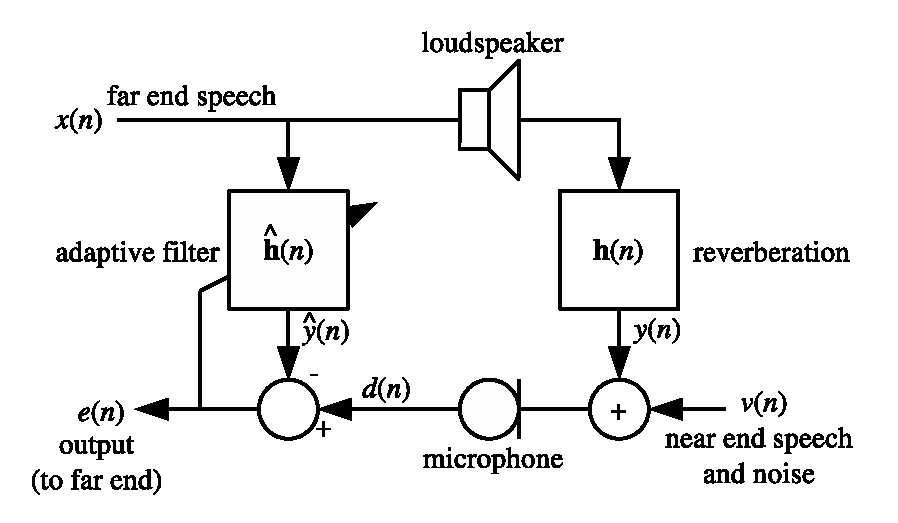
\includegraphics[width=10cm]{echo_path}\end{center}

\caption{Акустическая модель эха\label{fig:Acoustic-echo-model}}
\end{figure}


\section{Устройство передискретизации}

В некоторых случаях может быть полезным конвертирование звука из одной
частоты дискретизации в другую. Существует несколько причин для этого.
Это может использоваться для смешивания потоков у которых разные частоты
дискретизации, для поддержки частот дискретизации, не поддерживаемых
звуковой картой, для перекодировки, и т.д. Поэтому теперь устройство
передискретизации это часть проекта Speex. Данное устройство может
быть использовано для конвертирования между любыми двумя произвольными
частотами дискретизации (соотношение должно быть рациональным числом),
а также существует контроль над соотношением сложности и качества.
Помните что устройство передискретизации вводит некоторую задержку
в звуковой поток, чей размер зависит от установки сложности устройства
передискретизации. Обратитесь к документации на API для того чтобы
узнать как получить точные значения задержек.

\section{Интеграция}

Знание о том как использовать каждый из компонентов не настолько полезно,
если мы не знаем где их использовать. Рисунок \ref{fig:Integration-VoIP}
показывает где каждый из компонентов может быть использован в типичном
VoIP клиенте. Компоненты из пунктирных линий опциональны, хотя они
могут быть полезны при некоторых обстоятельствах. Существует несколько
моментов, о которых следует здесь упомянуть. AEC должен быть размещен
настолько близко насколько это возможно к воспроизводящей цепи и цепи
захвата. Только передискретизация может быть расположена него. Также
очень важно использовать одинаковое тактирование для захвата с микрофона
и воспроизведения на динамиках/наушниках.

\begin{figure}
\begin{center}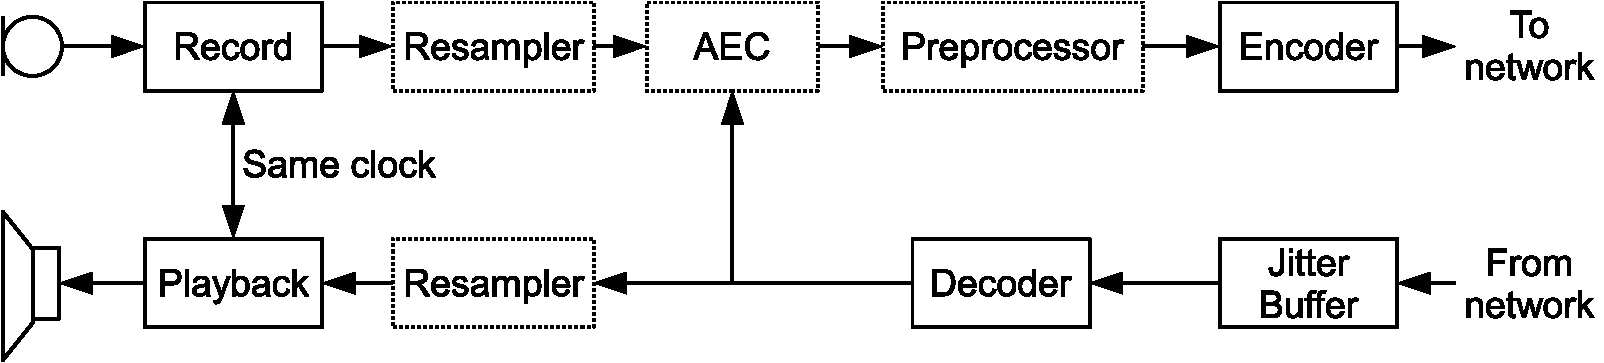
\includegraphics[width=0.8\textwidth]{components}\end{center}

\caption{Интеграция всех компонентов в VoIP клиенте.\label{fig:Integration-VoIP}}
\end{figure}

\newpage{}

\chapter{Компилирование и портирование}

Компилирование Speex под UNIX/Linux или множестве других платформ
поддерживающих autoconf (например Win32/cygwin) с легкостью осуществляется
путем написания:
\begin{lyxcode}
\%~./configure~{[}options{]}

\%~make

\%~make~install
\end{lyxcode}
Опции, поддерживаемые конфигурационным сценарием:
\begin{description}
\item [{--prefix=\textless path\textgreater}] Определяет путь установки
Speex (например /usr)
\item [{--enable-shared/--disable-shared}] Компилировать или не компилировать
разделяемые библиотеки
\item [{--enable-static/--disable-static}] Компилировать или не компилировать
статические библиотеки
\item [{--disable-wideband}] Отключить широкополосную часть Speex (обычно
для экономии памяти)
\item [{--enable-valgrind}] Enable extra hit for valgrind for debugging
purposes (не используется по умолчанию)
\item [{--enable-sse}] Включить использование инструкций SSE (только для
x86/float)
\item [{--enable-fixed-point\index{fixed-point}}] Компилировать для процессора
без (FPU)
\item [{--enable-arm4-asm}] Включить ассемблерную оптимизацию для архитектуры
ARMv4 (только для gcc)
\item [{--enable-arm5e-asm}] Включить ассемблерную оптимизацию для архитектуры
ARMv5E (только для gcc)
\item [{--enable-fixed-point-debug}] Используется только для отладки целочисленного\index{fixed-point}
кода (очень медленная)
\item [{--enable-ti-c55x}] Включить поддержку семейства TI C5x
\item [{--enable-blackfin-asm}] Включить ассемблерную оптимизацию для
архитектуры Blackfin DSP (только для gcc)
\end{description}

\section{Платформы}

Speex известен как компилируемый и работающий на множестве платформ
и архитектур, для чисел с плавающей точкой и фиксированной точкой.
В целом, любая архитектура, которая изначально может осуществлять
умножение для двух знаковых 16 разрядных чисел (с 32-х битным результатом)
и работать на достаточной тактовой частоте способна запустить Speex.
Архитектуры на которых замечена работоспособность Speex (может работать
на множестве других):
\begin{itemize}
\item x86 \& x86-64
\item Power
\item SPARC
\item ARM
\item Blackfin
\item Coldfire (семейство 68k)
\item TI C54xx \& C55xx
\item TI C6xxx
\item TriMedia (экспериментально)
\end{itemize}
Операционные системы на которых на которых замечена работоспособность
Speex включают в себя (может работать на множестве других):
\begin{itemize}
\item Linux
\item $\mu$Clinux
\item MacOS X
\item BSD
\item Остальные UNIX/POSIX системы
\item Symbian
\end{itemize}
Директория с исходным кодом включает в себя дополнительную информацию
о компилировании на определенных архитектурах и операционных системах
в файлах README.xxx.

\section{Портирование и оптимизация}

Здесь описаны некоторые моменты, рассматриваемые при портировании
или оптимизации Speex для новой или уже существующей платформы.

\subsection{Оптимизация программы}

Единственный фактор который значительно влияет на использование процессора
кодеком Speex состоит в том, скомпилирован ли он для вычислений с
плавающей точкой или с фиксированной. Если ваш ЦПУ/ЦСП не имеет модуля
обработки чисел с плавающей точкой, тогда скомпилированный с фиксированной
точкой кодек будет на порядки быстрее. На x86 архитектуре, вариант
с плавающей точкой \textbf{в основном} быстрее, но не всегда. Для
того, чтобы скомпилировать целочисленный вариант Speex, необходимо
передать параметр --fixed-point конфигурационному сценарию или определить
макрос FIXED\_POINT для компилятора. По состоянию на 1.2beta3, теперь
появилась возможность выключить API совместимости с плавающей точкой,
это означает, что программа будет подключаться без библиотеки эмуляции
плавающей точки. Для того чтобы это сделать, запустите конфигурацию
с параметром --disable-float-api или определите макрос DISABLE\_FLOAT\_API.
До тех пор пока функция VBR не портирована для целочисленного варианта,
вам также необходимо запускать конфигурацию с параметром --disable-vbr
или определить макрос DISABLE\_VBR.

Остальные важные моменты, которые необходимо проверить на некоторых
архитектурах сигнальных процессоров:
\begin{itemize}
\item Убедитесь в том что кэш установлен в режим с отложенной записью
\item Если чип имеет статическое ОЗУ вместо кэша, убедитесь сколько кода
и данных содержится в статическом ОЗУ, а не в ОЗУ
\end{itemize}
Если вы собираетесь писать на ассемблере, следующие функции обычно
необходимо рассматривать для оптимизации в первую очередь:
\begin{itemize}
\item \inputencoding{koi8-r}\lstinline!filter_mem16()!\inputencoding{utf8}
\item \inputencoding{koi8-r}\lstinline!iir_mem16()!\inputencoding{utf8}
\item \inputencoding{koi8-r}\lstinline!vq_nbest()!\inputencoding{utf8}
\item \inputencoding{koi8-r}\lstinline!pitch_xcorr()!\inputencoding{utf8}
\item \inputencoding{koi8-r}\lstinline!interp_pitch()!\inputencoding{utf8}
\end{itemize}
Функции фильтров \inputencoding{koi8-r}\lstinline!filter_mem16()!\inputencoding{utf8}
и \inputencoding{koi8-r}\lstinline!iir_mem16()!\inputencoding{utf8}
реализованы в виде транспонированной прямой формы второго типа (DF2T).
Хотя для архитектур, основанных умножении с накоплением (MAC), DF2T
требует частой перезагрузки аккумулятора, что может сделать программу
очень медленной. Для данных архитектур (т.е. Blackfin и Coldfire),
лучший подход состоит в применении первой прямой формы (DF1), который
проще выражается в элементах MAC. Важно убедиться в том, реализация
DF1 ведет себя также как оригинальная реализация DF2T при записи значений
в память. Это необходимо потому что фильтр меняющийся во времени и
должен вычислить точно такое же значение (без учета ошибки округления)
на кодировщике и декодировщике. 

\subsection{Оптимизация памяти}

Оптимизация памяти это то, что большей частью должно учитываться для
малых встраиваемых платформ. Для ПК Speex уже настолько мал что не
стоит делать вещей предлагаемых здесь. Существует несколько способов
уменьшить использование памяти в Speex, как для объема кода, так и
для объема данных. Для оптимизации объема кода трюк состоит в удалении
ненужных вам функций. Некоторые функции могут быть с легкостью удалены
если вы не нуждаетесь в них:
\begin{itemize}
\item Поддержка широкополосного режима (--disable-wideband)
\item Поддержка стерео (удаление stereo.c)
\item поддержка VBR (--disable-vbr или DISABLE\_VBR)
\item Статические кодовые таблицы которые не нужны, для битрейтов, которые
вы не используете ({*}\_table.c files)
\end{itemize}
У Speex также имеется несколько методов для размещения временных массивов.
При использовании компилятора, который поддерживает C99 (по состоянию
на 2007 год, компиляторы Microsoft не поддерживают, но gcc поддерживает),
лучше всего будет определить VAR\_ARRAYS. Это разрешит использование
функции массивов переменной длины C99. Следующим полезным шагом является
определение USE\_ALLOCA, в этом случае Speex будет использовать alloca()
для выделения памяти для временных массивов. Заметим что во множестве
систем, alloca() работает с ошибками и может не работать вовсе. Если
VAR\_ARRAYS и USE\_ALLOCA не определены, тогда Speex возвращается
к выделению больших ``временных областей'' и внутреннему разделению
выделенной памяти. Основной недостаток данного решения состоит в том
что оно требует много ресурсов. Необходимо выделить достаточно памяти
для худшего сценария (худший битрейт, наивысший параметр сложности,
...) и по умолчанию память не разделяется между множеством состояний
кодировщика/декодировщика. Тем не менее, если ручное выделение памяти
является единственным оставшимся вариантом, существует несколько моментов,
которые могут быть улучены. Переопределяя вызов функции the speex\_alloc\_scratch()
в os\_support.h, зачастую можно возвращать одну и ту же память для
всех состояний\footnote{В этом случае нужно быть осторожным с потоками}.
Вдобавок к этому, переопределением NB\_ENC\_STACK и NB\_DEC\_STACK
(или подобных для широкополосного режима), возможно выделить память
только для того сценария, который известен ранее. В этом случае важно
измерить количество памяти необходимого для определенной частоты выборок,
битрейта и уровня сложности который используется.

\newpage{}

\chapter{Консольные кодировщик и декодировщик\label{sec:Command-line-encoder/decoder}}

Базовый дистрибутив Speex включает в себя консольный кодировщик (\emph{speexenc})
и декодировщик (\emph{speexdec}). Эти инструменты создают и читают
файлы Speex, упакованные в контейнере Ogg. Хотя возможно инкапсулировать
Speex в любой контейнер, Ogg является рекомендуемым контейнером для
подобных файлов. Данный раздел рассказывает о том, как использовать
инструменты командной строки для файлов Speex в контейнере Ogg.

\section{\emph{speexenc\index{speexenc}}}

Утилита \emph{speexenc} используется для создания файлов Speex из
raw PCM или wave файлов. Функцией можно воспользоваться путем вызова: 
\begin{lyxcode}
speexenc~{[}опции{]}~входной\_файл~выходной\_файл
\end{lyxcode}
Значение '-' для входного\_файла или выходного\_файла соответствует
stdin и stdout соответственно. Доступны следующие опции:
\begin{description}
\item [{--narrowband~(-n)}] Включает обработку входного потока как узкополосного
(8 кГц). Эта опция установлена по умолчанию.
\item [{--wideband~(-w)}] Включает обработку входного потока как широкополосного
(16 кГц).
\item [{--ultra-wideband~(-u)}] Включает обработку входного потока как
ультра широкополосного (8 кГц).
\item [{--quality~n}] Устанавливает качество кодирования (0-10), по умолчанию
8
\item [{--bitrate~n}] Кодируемый битрейт (использует bit-rate n или ниже) 
\item [{--vbr}] Включить VBR (переменный битрейт), по умолчанию отключен
\item [{--abr~n}] Включить ABR (средний битрейт) равный n кбит/с, по
умолчанию отключен
\item [{--vad}] Включить VAD (определение присутствия голосового сигнала),
по умолчанию отключен
\item [{--dtx}] Включить DTX (прерывистая передача), по умолчанию отключена
\item [{--nframes~n}] Упаковывать n кадров в каждый Ogg пакет (это экономит
память на низких битрейтах)
\item [{--comp~n}] Установить соотношение скорости/качества. Более высокое
значение n замедляет кодирование (по умолчанию 3)
\item [{-V}] Подробный режим, показывает битрейт, используемый в данный
момент
\item [{--help~(-h)}] Вывести на экран помощь
\item [{--version~(-v)}] Показать информацию о версии ПО
\end{description}

\subsection*{Комментарии Speex}
\begin{description}
\item [{--comment}] Добавить данную строку как дополнительный комментарий.
Может быть использовано несколько раз. 
\item [{--author}] Автор трека.
\item [{--title}] Заголовок трека. 
\end{description}

\subsection*{Опции входных raw файлов}
\begin{description}
\item [{--rate~n}] Частота дискретизации входного потока
\item [{--stereo}] Рассматривать входной поток как стерео
\item [{--le}] Входной поток с прямым порядком бит 
\item [{--be}] Входной поток с обратным порядком бит 
\item [{--8bit}] Входной поток 8 бит беззнаковый
\item [{--16bit}] Входной поток 16 бит знаковый
\end{description}

\section{\emph{speexdec\index{speexdec}}}

Утилита \emph{speexdec} используется для декодирования файлов Speex
и может быть использована путем вызова: 
\begin{lyxcode}
speexdec~{[}опции{]}~speex\_файл~{[}выходной\_файл{]}
\end{lyxcode}
Значение '-' для speex\_файл или выходной\_файл соответствует stdin
и stdout. Также, когда не определен выходной файл, файл воспроизводится
через звуковую карту. Доступны следующие опции:
\begin{description}
\item [{--enh}] Включить фильтр (значение по умолчанию)
\item [{--no-enh}] Выключить фильтр
\item [{--force-nb}] Установить декодирование в узкополосном режиме 
\item [{--force-wb}] Установить декодирование в широкополосном режиме 
\item [{--force-uwb}] Установить декодирование в ультра широкополосном
режиме
\item [{--mono}] Установить декодирование в режиме моно 
\item [{--stereo}] Установить декодирование в режиме стерео 
\item [{--rate~n}] Установить декодирование на частоте дискретизации
n Гц
\item [{--packet-loss~n}] Имитировать n \% случайной потери пакетов
\item [{-V}] Подробный режим, показывает битрейт, используемый в данный
момент
\item [{--help~(-h)}] Вывести на экран помощь
\item [{--version~(-v)}] Показать информацию о версии ПО
\end{description}
\newpage{}

\chapter{Использование API кодека Speex (\emph{libspeex}\index{libspeex})\label{sec:Programming-with-Speex}}

Библиотека \emph{libspeex} содержит все функции для кодирования и
декодирования речи с использованием кодека Speex. При подключении
в операционных системах UNIX необходимо добавить \emph{-lspeex -lm}
в командную строку компилятора. Одна важная вещь которую необходимо
знать, это то что вызовы функций libspeex могут быть сделаны повторно,
\textbf{но при этом данная библиотека не ориентирована на многопоточное
исполнение}. Это означает, что нужно быть осторожным при вызове из
нескольких потоков, но \textbf{вызовы использующие одинаковое состояние
из нескольких потоков должны быть защищены мьютексами}. Примеры программ
также могут быть найдены в приложении \ref{sec:Sample-code} и полная
документация по API включена в раздел Documentation на сайте Speex
(http://www.speex.org/).

\section{Кодирование\label{subsec:Encoding}}

Для того, чтобы кодировать речь с использованием Speex, во-первых
необходимо:

\inputencoding{koi8-r}\begin{lstlisting}
#include <speex/speex.h>
\end{lstlisting}
\inputencoding{utf8}Далее в программе должна быть объявлена структура упаковщика битов
Speex вместе с переменной состояния кодировщика Speex:\inputencoding{koi8-r}
\begin{lstlisting}
SpeexBits bits;
void *enc_state;
\end{lstlisting}
\inputencoding{utf8}Во вторых, для инициализации:\inputencoding{koi8-r}
\begin{lstlisting}
speex_bits_init(&bits);
enc_state = speex_encoder_init(&speex_nb_mode);
\end{lstlisting}
\inputencoding{utf8}
Для широкополосного режима, \emph{speex\_nb\_mode} должна быть заменена
\emph{speex\_wb\_mode}. В большинстве случаев, вам необходимо знать
размер кадра при используемой вами частоте дискретизации. Вы можете
получить это значение через переменную \emph{frame\_size} (выраженную
в выборках, а не в байтах) с помощью:

\inputencoding{koi8-r}\begin{lstlisting}
speex_encoder_ctl(enc_state,SPEEX_GET_FRAME_SIZE,&frame_size);
\end{lstlisting}
\inputencoding{utf8}
На практике, \emph{frame\_size} должен соответствовать 20 миллисекундам
при использовании частоты дискретизации в 8, 16, или 32 кГц. Существует
множество параметров, которые должны быть установлены для кодировщика
Speex, но наиболее полезный из них это параметр качества, который
контролирует соотношение между качеством и битрейтом. Он устанавливается
с помощью:

\inputencoding{koi8-r}\begin{lstlisting}
speex_encoder_ctl(enc_state,SPEEX_SET_QUALITY,&quality);
\end{lstlisting}
\inputencoding{utf8}где \emph{quality} это целое число между 0 и 10 (включительно). Соотношение
между качеством и битрейтом показано на рисунке \ref{cap:quality_vs_bps}
для узкополосного режима.

После того как инициализация произведена, для каждого входящего кадра:

\inputencoding{koi8-r}\begin{lstlisting}
speex_bits_reset(&bits);
speex_encode_int(enc_state, input_frame, &bits);
nbBytes = speex_bits_write(&bits, byte_ptr, MAX_NB_BYTES);
\end{lstlisting}
\inputencoding{utf8}
где \emph{input\_frame} это \emph{(}short \emph{{*})} указатель на
начало речевого кадра, \emph{byte\_ptr} это \emph{(char {*})} это
указатель на начало закодированного кадра, \emph{MAX\_NB\_BYTES} это
максимальное число байт, которые могут быть записаны в \emph{byte\_ptr,}
не вызывая переполнения стека, и \emph{nbBytes} это число байт, которое
записано в \emph{byte\_ptr} (размер закодированного кадра в байтах).
До вызова speex\_bits\_write, можно определить количество байт, которые
будут записаны, с помощью вызова \texttt{speex\_bits\_nbytes(\&bits)},
которая возвращает количество байт.

Возможно использование функции \emph{speex\_encode()}, которая использует
\emph{(float {*})} для звука. Хотя это может сделать порт на платформу
без модуля обработки операций с плавающей точкой (например ARM) более
медленным. Внутренне \emph{speex\_encode()} и \emph{speex\_encode\_int()}
работают одинаково. Использование кодировщиком целочисленного варианта
или варианта с плавающей точкой определяется только флагами компилятора,
а не на уровне API.

После того, как вы выполнили кодирование, освободите ресурсы через:

\inputencoding{koi8-r}\begin{lstlisting}
speex_bits_destroy(&bits);
speex_encoder_destroy(enc_state);
\end{lstlisting}
\inputencoding{utf8}

\section{Декодирование\label{subsec:Decoding}}

Для декодирования речи с использованием Speex, сначала вам нужно:\inputencoding{koi8-r}
\begin{lstlisting}
#include <speex/speex.h>
\end{lstlisting}
\inputencoding{utf8}Также необходимо объявить структуру\inputencoding{koi8-r}
\begin{lstlisting}
SpeexBits bits;
\end{lstlisting}
\inputencoding{utf8}и переменную состояния декодера \inputencoding{koi8-r}
\begin{lstlisting}
void *dec_state;
\end{lstlisting}
\inputencoding{utf8}Они инициализируются с помощью:\inputencoding{koi8-r}
\begin{lstlisting}
speex_bits_init(&bits);
dec_state = speex_decoder_init(&speex_nb_mode);
\end{lstlisting}
\inputencoding{utf8}
Для широкополосного режима, \emph{speex\_nb\_mode} должна быть заменена
\emph{speex\_wb\_mode}. В большинстве случаев, вам необходимо знать
размер кадра при используемой вами частоте дискретизации. Вы можете
получить это значение через переменную \emph{frame\_size} (выраженную
в выборках, а не байтах) с помощью:

\inputencoding{koi8-r}\begin{lstlisting}
speex_decoder_ctl(dec_state, SPEEX_GET_FRAME_SIZE, &frame_size);
\end{lstlisting}
\inputencoding{utf8}
Также существует параметр, который должен быть установлен для декодировщика:
используется ли перцепционный усилитель или нет. Он должен быть установлен
с помощью: 

\inputencoding{koi8-r}\begin{lstlisting}
speex_decoder_ctl(dec_state, SPEEX_SET_ENH, &enh);
\end{lstlisting}
\inputencoding{utf8}
где \emph{enh} целое значение равное 0 для выключения усилителя и
1 для включения. Для 1.2-beta1, по умолчанию он включен.

Опять, после того как инициализация декодера завершена, для каждого
входящего кадра:

\inputencoding{koi8-r}\begin{lstlisting}
speex_bits_read_from(&bits, input_bytes, nbBytes);
speex_decode_int(dec_state, &bits, output_frame);
\end{lstlisting}
\inputencoding{utf8}где input\_bytes это \emph{(char {*})} содержащий потоковые данные
для одного кадра, \emph{nbBytes} размер (в байтах) этого потока, и
\emph{output\_frame} это \emph{(short {*})} которое указывает на область,
в которой будут записаны декодированные речевые кадры. Значение NULL
в качестве второго аргумента показывает что у нас нету данных для
текущего кадра. Когда кадр теряется, декодер Speex пытается угадать
правильный сигнал.

Как и для кодировщика, функция \emph{speex\_decode()} также может
быть использована с \emph{(float {*}),} как выходными данными для
звука. После того как вы завершили декодирование, освободите все ресурсы
с помощью:

\inputencoding{koi8-r}\begin{lstlisting}
speex_bits_destroy(&bits);
speex_decoder_destroy(dec_state);
\end{lstlisting}
\inputencoding{utf8}

\section{Опции кодека (speex\_{*}\_ctl)\label{subsec:Codec-Options}}
\begin{quote}
\begin{center}
\emph{Entities should not be multiplied beyond necessity -- William
of Ockham. }
\par\end{center}
\begin{center}
\emph{Just because there’s an option for it doesn’t mean you have
to turn it on -- me. }
\par\end{center}

\end{quote}
Кодировщик и декодировщик Speex поддерживают множество опций и запросов,
которые могут быть доступны через функции\emph{ speex\_encoder\_ctl}
и \emph{speex\_decoder\_ctl}. Эти функции схожи с системными вызовами
\emph{ioctl} и их прототипы имеют следующий вид:

\inputencoding{koi8-r}\begin{lstlisting}
void speex_encoder_ctl(void *encoder, int request, void *ptr);
void speex_decoder_ctl(void *encoder, int request, void *ptr);
\end{lstlisting}
\inputencoding{utf8}
Несмотря на наличие этих функций, значения по умолчанию обычно подходят
для большинства приложений и опциональные настройки \textbf{могут
быть использованы только тогда, когда вы понимаете что они означают,
и знаете для чего они вам нужны.} Основная ошибка состоит в попытке
установить множество ненужных настроек. 

Здесь представлен список значений, применяемых для запросов. Некоторые
из них применяются только для кодировщика или декодировщика. Потому
как последний аргумент имеет тип \inputencoding{koi8-r}\lstinline!void *!\inputencoding{utf8},
функции \inputencoding{koi8-r}\lstinline!_ctl()!\inputencoding{utf8}
не типобезопасны, таким образом вы должны их использовать с осторожностью.
Тип \inputencoding{koi8-r}\lstinline!spx_int32_t!\inputencoding{utf8}
это тип \inputencoding{koi8-r}\lstinline!int32_t!\inputencoding{utf8}
в C99.
\begin{description}
\item [{SPEEX\_SET\_ENH$\ddagger$}] Установить перцепционный усилитель\index{perceptual enhancement}
для включения (1) или (0) для того чтобы выключить (\inputencoding{koi8-r}\lstinline!spx_int32_t!\inputencoding{utf8},
по умолчанию включен)
\item [{SPEEX\_GET\_ENH$\ddagger$}] Получить статус перцепционного усилителя
(\inputencoding{koi8-r}\lstinline!spx_int32_t!\inputencoding{utf8})
\item [{SPEEX\_GET\_FRAME\_SIZE}] Получить количество выборок на кадр текущем
режиме (\inputencoding{koi8-r}\lstinline!spx_int32_t!\inputencoding{utf8})
\item [{SPEEX\_SET\_QUALITY$\dagger$}] Установить качество кодируемой
речи (\inputencoding{koi8-r}\lstinline!spx_int32_t!\inputencoding{utf8}
от 0 до 10, по умолчанию 8)
\item [{SPEEX\_GET\_QUALITY$\dagger$}] Получить текущее значение качества
кодируемой речи (\inputencoding{koi8-r}\lstinline!spx_int32_t!\inputencoding{utf8}
от 0 до 10)
\item [{SPEEX\_SET\_MODE$\dagger$}] Установить режим под номером, как
определено в RTP спецификации (\inputencoding{koi8-r}\lstinline!spx_int32_t!\inputencoding{utf8})
\item [{SPEEX\_GET\_MODE$\dagger$}] Получить режим под номером, как определено
в RTP спецификации (\inputencoding{koi8-r}\lstinline!spx_int32_t!\inputencoding{utf8})
\item [{SPEEX\_SET\_VBR$\dagger$}] Установить переменный битрейт (VBR)
(1) чтобы включить, (0) чтобы выключить (\inputencoding{koi8-r}\lstinline!spx_int32_t!\inputencoding{utf8},
по умолчанию выключен)
\item [{SPEEX\_GET\_VBR$\dagger$}] Получить статус переменного битрейта
\index{variable bit-rate} (VBR) (\inputencoding{koi8-r}\lstinline!spx_int32_t!\inputencoding{utf8})
\item [{SPEEX\_SET\_VBR\_QUALITY$\dagger$}] Установить качество кодируемой
речи при включенном VBR (float 0.0 до 10.0, по умолчанию 8.0)
\item [{SPEEX\_GET\_VBR\_QUALITY$\dagger$}] Получить значение качества
кодируемой речи при включенном VBR (float от 0 до 10)
\item [{SPEEX\_SET\_COMPLEXITY$\dagger$}] Установить ресурсы ЦПУ, разрешенные
для кодировщика (\inputencoding{koi8-r}\lstinline!spx_int32_t!\inputencoding{utf8}
от 1 до 10, по умолчанию 2)
\item [{SPEEX\_GET\_COMPLEXITY$\dagger$}] Получить ресурсы ЦПУ, разрешенные
для кодировщика (\inputencoding{koi8-r}\lstinline!spx_int32_t!\inputencoding{utf8}
от 1 до 10)
\item [{SPEEX\_SET\_BITRATE$\dagger$}] Установить битрейт, использует
ближайшее значение, не превышающее параметр (\inputencoding{koi8-r}\lstinline!spx_int32_t!\inputencoding{utf8}
в битах в секунду)
\item [{SPEEX\_GET\_BITRATE}] Получить текущий используемый битрейт (\inputencoding{koi8-r}\lstinline!spx_int32_t!\inputencoding{utf8}
в битах в секунду)
\item [{SPEEX\_SET\_SAMPLING\_RATE}] Установить частоту дискретизации (\inputencoding{koi8-r}\lstinline!spx_int32_t!\inputencoding{utf8}
в Гц)
\item [{SPEEX\_GET\_SAMPLING\_RATE}] Получить частоту дискретизации (\inputencoding{koi8-r}\lstinline!spx_int32_t!\inputencoding{utf8}
в Гц)
\item [{SPEEX\_RESET\_STATE}] Сбросить состояние кодировщика/декодировщика,
стирает всю память (без аргумента)
\item [{SPEEX\_SET\_VAD$\dagger$}] Установить значение определения присутствия
голосового сигнала\index{voice activity detection} (VAD), (1) чтобы
включить, (0) чтобы выключить (\inputencoding{koi8-r}\lstinline!spx_int32_t!\inputencoding{utf8},
по умолчанию выключен)
\item [{SPEEX\_GET\_VAD$\dagger$}] Получить статус определения присутствия
голосового сигнала (VAD) (\inputencoding{koi8-r}\lstinline!spx_int32_t!\inputencoding{utf8})
\item [{SPEEX\_SET\_DTX$\dagger$}] Установить прерывистую передачу \index{discontinuous transmission}
(DTX), (1) чтобы включить, (0) чтобы выключить (\inputencoding{koi8-r}\lstinline!spx_int32_t!\inputencoding{utf8},
по умолчанию выключен)
\item [{SPEEX\_GET\_DTX$\dagger$}] Получить статус прерывистой передачи
(DTX) (\inputencoding{koi8-r}\lstinline!spx_int32_t!\inputencoding{utf8})
\item [{SPEEX\_SET\_ABR$\dagger$}] Установить значение среднего битрейта
при \index{average bit-rate} (ABR) в бит в секунду (\inputencoding{koi8-r}\lstinline!spx_int32_t!\inputencoding{utf8}
в битах в секунду)
\item [{SPEEX\_GET\_ABR$\dagger$}] Получить значение среднего битрейта
при (ABR) (\inputencoding{koi8-r}\lstinline!spx_int32_t!\inputencoding{utf8}
в битах в секунду)
\item [{SPEEX\_SET\_PLC\_TUNING$\dagger$}] Сказать кодировщику оптимизировать
кодирование для определенного процента потери пакетов (\inputencoding{koi8-r}\lstinline!spx_int32_t!\inputencoding{utf8}
в процентах)
\item [{SPEEX\_GET\_PLC\_TUNING$\dagger$}] Получить текущее значение PLC
(\inputencoding{koi8-r}\lstinline!spx_int32_t!\inputencoding{utf8}
в процентах)
\item [{SPEEX\_GET\_LOOKAHEAD}] Возвращает lookahead используемый Speex
отдельно для кодировщика и декодировщика. Сумма значений lookahead
кодировщика и декодировщика это общее значение lookahead.
\item [{SPEEX\_SET\_VBR\_MAX\_BITRATE$\dagger$}] Установить максимальный
битрейт допустимый при использовании VBR (\inputencoding{koi8-r}\lstinline!spx_int32_t!\inputencoding{utf8}
в битах в секунду)
\item [{SPEEX\_GET\_VBR\_MAX\_BITRATE$\dagger$}] Получить максимальный
битрейт допустимый при использовании VBR (\inputencoding{koi8-r}\lstinline!spx_int32_t!\inputencoding{utf8}
в битах в секунду)
\item [{SPEEX\_SET\_HIGHPASS}] Установить фильтр верхних частот в (1) или
выключить (0) (\inputencoding{koi8-r}\lstinline!spx_int32_t!\inputencoding{utf8},
по умолчанию включен)
\item [{SPEEX\_GET\_HIGHPASS}] Получить текущий статус фильтра верхних
частот (\inputencoding{koi8-r}\lstinline!spx_int32_t!\inputencoding{utf8})
\item [{$\dagger$}] применяются только для кодировщика
\item [{$\ddagger$}] применяются только для декодировщика
\end{description}

\section{Запросы режима\label{subsec:Mode-queries}}

Режимы Speex имеют систему запросов похожую на speex\_encoder\_ctl
и speex\_decoder\_ctl. Так как режимы доступны только для чтения,
возможно только получать информацию о конкретном режиме. Функция осуществляющая
это представлена ниже:\inputencoding{koi8-r}
\begin{lstlisting}
void speex_mode_query(SpeexMode *mode, int request, void *ptr);
\end{lstlisting}
\inputencoding{utf8}Допустимые значения для запросов следующие (если не указано иное,
значения возвращаются через \emph{ptr}):
\begin{description}
\item [{SPEEX\_MODE\_FRAME\_SIZE}] Получить размер кадра (в выборках) для
режима
\item [{SPEEX\_SUBMODE\_BITRATE}] Получить битрейт для подрежима определенного
через \emph{ptr} (целое в бит/с). 
\end{description}

\section{Формирование пакетов и внутридиапазонная связь\index{in-band signalling}}

Иногда желательно разместить больше одного кадра на каждый пакет (или
другую базовую единицу хранения данных). Правильный способ сделать
это, это вызвать speex\_encode $N$ раз до записи потока с помощью
speex\_bits\_write. В случаях где количество кадров не определено
внеполосным механизмом, возможно включить код разделителя. Данный
разделитель состоит из кода 15 (в десятичной системе счисления) закодированного
пятью битами, как показано в таблице \ref{cap:quality_vs_bps}. Заметим
что на момент версии 1.0.2, вызов speex\_bits\_write автоматически
вставляет разделитель к моменту заполнения последнего байта. Он не
включает в себя какого либо заголовка, поэтому убедитесь, что Speex
всегда определяет момент, когда нет больше кадров в пакете.

Также возможно отправить внутридиапазонные ``сообщения'' другой
стороне. Все данные сообщения кодируются как псевдо кадры режима 14,
который содержит 4-х битовый код типа сообщения с последующим сообщением.
Таблица \ref{cap:In-band-signalling-codes} содержит список допустимых
кодов, их значение и размер сообщения, следующего после. Большинство
из этих сообщений это запросы, которые отправляются кодировщику или
декодировщику на другой конец, который может соблюдать или игнорировать
их. По умолчанию все внутридиапазонные сообщения игнорируются. 

\begin{table}[htbp]
\begin{center}%
\begin{tabular}{|c|c|c|}
\hline 
Код & Размер (бит) & Содержимое\tabularnewline
\hline 
\hline 
0 & 1 & Запрашивает у декодировщика установить перцепционное усиление выключенным
(0) или включенным (1)\tabularnewline
\hline 
1 & 1 & Запрашивает (если 1) у кодировщика быть менее ``агрессивным'' к
большим потерям пакетов\tabularnewline
\hline 
2 & 4 & Запрашивает у кодировщика переключится в режим N\tabularnewline
\hline 
3 & 4 & Запрашивает у кодировщика переключится в режим N для нижнего диапазона\tabularnewline
\hline 
4 & 4 & Запрашивает у кодировщика переключится в режим N для верхнего диапазона\tabularnewline
\hline 
5 & 4 & Запрашивает у кодировщика переключится на качество N для VBR\tabularnewline
\hline 
6 & 4 & Запросить подтверждение (0=нет, 1=все, 2=только для внутридиапазонных
данных)\tabularnewline
\hline 
7 & 4 & Запрашивает у кодировщика установить CBR (0), VAD(1), DTX(3), VBR(5),
VBR+DTX(7)\tabularnewline
\hline 
8 & 8 & Передать (восьмиразрядное) значение в другой конец\tabularnewline
\hline 
9 & 8 & Информация об интенсивности стерео\tabularnewline
\hline 
10 & 16 & Объявить максимально допустимый битрейт (N в байтах в секунду)\tabularnewline
\hline 
11 & 16 & зарезервировано\tabularnewline
\hline 
12 & 32 & Подтверждение приема пакета N\tabularnewline
\hline 
13 & 32 & зарезервировано\tabularnewline
\hline 
14 & 64 & зарезервировано\tabularnewline
\hline 
15 & 64 & зарезервировано\tabularnewline
\hline 
\end{tabular}\end{center}

\caption{Коды внутридиапазонной связи\label{cap:In-band-signalling-codes}}
\end{table}

Наконец, приложения могут определять собственные внутридиапазонные
сообщения, используя режим 13. Размер сообщения в байтах кодируется
пятью битами, так что декодировщик может пропустить их, если не знает
как их интерпретировать.\newpage{}

\chapter{API обработки звука (\emph{libspeexdsp})}

На момент версии 1.2beta3, части пакета Speex, не относящиеся к кодеку,
теперь расположены в отдельной библиотеке названной \emph{libspeexdsp}.
Данная библиотека включает в себя препроцессор, акустическое подавление
эха, буфер колебаний задержки, и устройство передискретизации. В среде
UNIX она может быть подключена к программе путем добавления \emph{-lspeexdsp
-lm} в командной строке компилятора. Также как и в случае с libspeex,
\textbf{вызовы libspeexdsp реентрабельны, но не потокобезопасны}.
Это означает что нужно быть осторожным при вызове из нескольких потоков,
но \textbf{вызовы, использующие одинаковое состояние из нескольких
потоков, должны быть защищены мьютексами.}

\section{Препроцессор\label{subsec:Preprocessor}}

\noindent Для того, чтобы использовать препроцессор Speex\index{preprocessor},
вам необходимо:\inputencoding{koi8-r}
\begin{lstlisting}
#include <speex/speex_preprocess.h>
\end{lstlisting}
\inputencoding{utf8}
\noindent После чего, состояние препроцессора может быть установлено
через:\inputencoding{koi8-r}
\begin{lstlisting}
SpeexPreprocessState *preprocess_state = speex_preprocess_state_init(frame_size, sampling_rate);
\end{lstlisting}
\inputencoding{utf8}
\noindent и рекомендуется использовать те значения \texttt{frame\_size},
которые использовались для кодировщика (20 мс).

Для каждого входящего кадра необходимо вызывать:

\inputencoding{koi8-r}\begin{lstlisting}
speex_preprocess_run(preprocess_state, audio_frame);
\end{lstlisting}
\inputencoding{utf8}
\noindent где \texttt{audio\_frame} используется и для входного и
для выходного потока. В случаях, когда нет полезного звука на выходе
в текущем кадре, можно использовать функцию:

\inputencoding{koi8-r}\begin{lstlisting}
speex_preprocess_estimate_update(preprocess_state, audio_frame);
\end{lstlisting}
\inputencoding{utf8}
\noindent Данный вызов обновит все внутренние переменные состояния
препроцессора без вычисления выходного звука, таким образом экономя
ресурсы процессора.

Поведение препроцессора может быть изменено с помощью:

\inputencoding{koi8-r}\begin{lstlisting}
speex_preprocess_ctl(preprocess_state, request, ptr);
\end{lstlisting}
\inputencoding{utf8}
\noindent которая используется так же как её эквивалент для кодировщика
и декодировщика. Опции описаны в разделе \ref{subsec:Preprocessor-options}.

Состояние препроцессора может быть уничтожено с помощью:

\inputencoding{koi8-r}\begin{lstlisting}
speex_preprocess_state_destroy(preprocess_state);
\end{lstlisting}
\inputencoding{utf8}

\subsection{Опции препроцессора\label{subsec:Preprocessor-options}}

Как и в случае с кодеком, препроцессор также имеет опции, которые
контролируются при помощи ioctl() подобных вызовов. Доступны следующие
опции:
\begin{description}
\item [{SPEEX\_PREPROCESS\_SET\_DENOISE}] Включает шумоподавление, (1)
чтобы включить, (0) чтобы выключить (\inputencoding{koi8-r}\lstinline!spx_int32_t!\inputencoding{utf8})
\item [{SPEEX\_PREPROCESS\_GET\_DENOISE}] Возвращает состояние устройства
шумоподавления (\inputencoding{koi8-r}\lstinline!spx_int32_t!\inputencoding{utf8})
\item [{SPEEX\_PREPROCESS\_SET\_AGC}] Включает автоматическую регулировку
усиления (AGC), (1) чтобы включить, (0) чтобы выключить (\inputencoding{koi8-r}\lstinline!spx_int32_t!\inputencoding{utf8})
\item [{SPEEX\_PREPROCESS\_GET\_AGC}] Возвращает состояние AGC (\inputencoding{koi8-r}\lstinline!spx_int32_t!\inputencoding{utf8})
\item [{SPEEX\_PREPROCESS\_SET\_VAD}] Включает детектор активности звука
(VAD), (1) чтобы включить, (0) чтобы выключить (\inputencoding{koi8-r}\lstinline!spx_int32_t!\inputencoding{utf8})
\item [{SPEEX\_PREPROCESS\_GET\_VAD}] Возвращает состояние VAD (\inputencoding{koi8-r}\lstinline!spx_int32_t!\inputencoding{utf8})
\item [{SPEEX\_PREPROCESS\_SET\_AGC\_LEVEL}]~
\item [{SPEEX\_PREPROCESS\_GET\_AGC\_LEVEL}]~
\item [{SPEEX\_PREPROCESS\_SET\_DEREVERB}] Включает удаление реверберации,
(1) чтобы включить, (0) чтобы выключить (\inputencoding{koi8-r}\lstinline!spx_int32_t!\inputencoding{utf8})
\item [{SPEEX\_PREPROCESS\_GET\_DEREVERB}] Возвращает состояние удалятора
реверберации (\inputencoding{koi8-r}\lstinline!spx_int32_t!\inputencoding{utf8})
\item [{SPEEX\_PREPROCESS\_SET\_DEREVERB\_LEVEL}] На данный момент не работает,
не используйте
\item [{SPEEX\_PREPROCESS\_GET\_DEREVERB\_LEVEL}] На данный момент не работает,
не используйте
\item [{SPEEX\_PREPROCESS\_SET\_DEREVERB\_DECAY}] На данный момент не работает,
не используйте
\item [{SPEEX\_PREPROCESS\_GET\_DEREVERB\_DECAY}] На данный момент не работает,
не используйте
\item [{SPEEX\_PREPROCESS\_SET\_PROB\_START}]~
\item [{SPEEX\_PREPROCESS\_GET\_PROB\_START}]~
\item [{SPEEX\_PREPROCESS\_SET\_PROB\_CONTINUE}]~
\item [{SPEEX\_PREPROCESS\_GET\_PROB\_CONTINUE}]~
\item [{SPEEX\_PREPROCESS\_SET\_NOISE\_SUPPRESS}] Устанавливает максимальное
подавление шума в дБ (отрицательное \inputencoding{koi8-r}\lstinline!spx_int32_t!\inputencoding{utf8})
\item [{SPEEX\_PREPROCESS\_GET\_NOISE\_SUPPRESS}] Возвращает максимальное
подавление шума в дБ (отрицательное \inputencoding{koi8-r}\lstinline!spx_int32_t!\inputencoding{utf8})
\item [{SPEEX\_PREPROCESS\_SET\_ECHO\_SUPPRESS}] Устанавливает максимальное
ослабление эха в дБ (отрицательное \inputencoding{koi8-r}\lstinline!spx_int32_t!\inputencoding{utf8})
\item [{SPEEX\_PREPROCESS\_GET\_ECHO\_SUPPRESS}] Возвращает максимальное
ослабление эха в дБ (отрицательное \inputencoding{koi8-r}\lstinline!spx_int32_t!\inputencoding{utf8})
\item [{SPEEX\_PREPROCESS\_SET\_ECHO\_SUPPRESS\_ACTIVE}] Устанавливает
максимальное ослабление эха в дБ, когда когда ближний конец активен
(отрицательное \inputencoding{koi8-r}\lstinline!spx_int32_t!\inputencoding{utf8})
\item [{SPEEX\_PREPROCESS\_GET\_ECHO\_SUPPRESS\_ACTIVE}] Возвращает максимальное
ослабление эха в дБ, когда когда ближний конец активен (отрицательное
\inputencoding{koi8-r}\lstinline!spx_int32_t!\inputencoding{utf8})
\item [{SPEEX\_PREPROCESS\_SET\_ECHO\_STATE}] Устанавливает связанный эхокомпенсатор
для остаточного подавления эха (указатель или NULL для отключения
подавления остаточного эха)
\item [{SPEEX\_PREPROCESS\_GET\_ECHO\_STATE}] Возвращает связанный эхокомпенсатор
(указатель)
\end{description}

\section{Подавление эха\label{subsec:Echo-Cancellation}}

Библиотека Speex на данный момент включает в себя алгоритм подавление
эха\index{echo cancellation} подходящий для эхоподавления\index{acoustic echo cancellation}
(AEC). В случае использования эхоподавления, в первую очередь необходимо:

\inputencoding{koi8-r}\begin{lstlisting}
#include <speex/speex_echo.h>
\end{lstlisting}
\inputencoding{utf8}
После чего режим эхоподавления должен быть установлен с помощью:

\inputencoding{koi8-r}\begin{lstlisting}
SpeexEchoState *echo_state = speex_echo_state_init(frame_size, filter_length);
\end{lstlisting}
\inputencoding{utf8}
где \texttt{frame\_size} это количество данных (в выборках), которые
необходимо вам обработать сразу, и \texttt{filter\_length} это размер
(в выборках) фильтра подавления эха который вы используете (также
известен как \textit{tail length}\index{tail length}). Рекомендуется
использовать размер кадра кратного 20 мс (или равного размеру кадра
кодека), и убедитесь в том, что FFT легко выполняется при данном размере
(степени двойки лучше чем остальные числа). Рекомендуемый размер фильтра
приблизительно равен одной трети времени отражения звука в помещении.
Например, в маленькой комнате, время отражения звука порядка 300 мс,
таким образом размер фильтра равный 100 мс (800 выборок при частоте
дискретизации в 8000 Гц) это правильный выбор.

После того, как режим подавления эха был остановлен, звук может отрабатываться
с помощью:

\inputencoding{koi8-r}\begin{lstlisting}
speex_echo_cancellation(echo_state, input_frame, echo_frame, output_frame);
\end{lstlisting}
\inputencoding{utf8}
где \texttt{input\_frame} это звук, который зафиксирован микрофоном,
\texttt{echo\_frame} это сигнал, который воспроизводится динамиками
(и должен быть убран) и \texttt{output\_frame} это сигнал с убранным
эхо. 

Одна важная вещь состоит в соотношении между \texttt{input\_frame}
и \texttt{echo\_frame}. Важно то, что в любое время любое эхо, которое
появляется на входе, было отправлено в фильтр эхоподавления как \texttt{echo\_frame}.
Другими словами, фильтр эхоподавления не может убрать сигнал, который
еще не принят. С другой стороны, задержка между входным сигналом и
сигналом эха должна быть достаточно малой, потому как иначе часть
фильтра эхоподавления будет работать впустую. В идеальном случае ваша
программа должна выглядеть так:\inputencoding{koi8-r}
\begin{lstlisting}[breaklines=true]
write_to_soundcard(echo_frame, frame_size);
read_from_soundcard(input_frame, frame_size);
speex_echo_cancellation(echo_state, input_frame, echo_frame, output_frame);
\end{lstlisting}
\inputencoding{utf8}
Если вы хотите в дальнейшем уменьшить эхо, представленное в сигнале,
вы должны сделать это путем связывания фильтра эхоподавления с препроцессором
(см. раздел \ref{subsec:Preprocessor}). Это осуществляется с помощью
вызова:\inputencoding{koi8-r}
\begin{lstlisting}[breaklines=true]
speex_preprocess_ctl(preprocess_state, SPEEX_PREPROCESS_SET_ECHO_STATE,echo_state);
\end{lstlisting}
\inputencoding{utf8}при инициализации.

На момент версии 1.2-beta2, существует альтернативный, более простой
API, который может быть использован вместо \emph{speex\_echo\_cancellation()}.
Когда захват звука и его воспроизведение обрабатывается асинхронно
(т.е. в разных потоках или с использованием системных вызовов \emph{poll()}
или \emph{select()} ), тогда будет сложно отследить, который input\_frame
пришел с каким из echo\_frame. Вместо этого, контекст или поток воспроизведения
может быть просто вызван через:

\inputencoding{koi8-r}\begin{lstlisting}
speex_echo_playback(echo_state, echo_frame);
\end{lstlisting}
\inputencoding{utf8}
каждый раз когда воспроизводится звуковой кадр. После чего захват
контекста/потока с помощью вызова:

\inputencoding{koi8-r}\begin{lstlisting}
speex_echo_capture(echo_state, input_frame, output_frame);
\end{lstlisting}
\inputencoding{utf8}
для каждого полученного кадра. Внутренне, \emph{speex\_echo\_playback()}
проще буферизирует воспроизводимый кадр, таким образом, этим можно
воспользоваться, вызвав \emph{speex\_echo\_capture()} для вызова \emph{speex\_echo\_cancel()}.
Побочный эффект использования альтернативного API состоит в том, что
воспроизводимый звук задерживается на два кадра, что является нормальной
задержкой, вызванной звуковой картой. Когда захват и воспроизведение
синхронизированы, \emph{speex\_echo\_cancellation()} предпочтительнее,
так как предоставляет лучший контроль при точном входном/эхо тайминге.

Состояние эхоподавления может быть удалено с помощью:

\inputencoding{koi8-r}\begin{lstlisting}
speex_echo_state_destroy(echo_state);
\end{lstlisting}
\inputencoding{utf8}
Также можно сбросить состояние эхоподавления, таким образом, оно может
быть использовано повторно без необходимости создания другого состояния,
с помощью:

\inputencoding{koi8-r}\begin{lstlisting}
speex_echo_state_reset(echo_state);
\end{lstlisting}
\inputencoding{utf8}

\subsection{Решение проблем}

Существует несколько вещей, которые могут препятствовать правильной
работе эхоподавления. Одна из них это ошибка (или нечто условно оптимальное)
в коде, но существует множество других ошибок, на которых вы должны
сосредоточиться в первую очередь.
\begin{itemize}
\item Использование разных звуковых карт для записи и воспроизведения не
будет работать, независимо от того, что вы можете подумать. Единственное
исключение состоит в том, что если две звуковые карты смогут зафиксировать
их тактовые частоты на одном источнике тактовой частоты. Если нет,
тогда тактовые частоты всегда будут иметь некоторый дрейф, который
предотвратит адаптацию фильтра эхоподавления.
\item Задержка между записью и воспроизведением сигналов должна быть минимальной.
Любой воспроизводимый сигнал должен появиться на воспроизводящем устройстве
(дальний конец) немного раньше, чем фильтр эхоподавления увидит его
в записанном сигнале, но чрезмерная задержка подразумевает, что часть
фильтра будет использовано впустую. В худших ситуациях задержка настолько
большая, что больше чем длина фильтра, в данном случае, никакое эхо
не будет подавляться.
\item Когда дело доходит до длины фильтра, длиннее не значит лучше. На самом
деле, при большей длине фильтра фильтр адаптируется дольше. Безусловно,
слишком маленькая длина фильтра не достаточна для подавления эха,
но наиболее распространенная проблема заключается в том что люди устанавливают
слишком большую длину фильтра и после удивляются тому, что эхо не
подавляется.
\item Нелинейные искажения не могут быть (по определению) смоделированы
линейным адаптивным фильтром, используемым в устройстве эхоподавления,
и также не могут быть подавлены. Используйте хороший звуковой тракт
и избежите насыщения/отсечения.
\end{itemize}
Также полезно прочесть \emph{Echo Cancellation Demystified} Алексея
Фрунзе\footnote{http://www.embeddedstar.com/articles/2003/7/article20030720-1.html},
которая объясняет фундаментальные принципы эхоподавления. Детали алгоритма
описанные в статье отличаются, но основные идеи эхоподавления через
адаптивные фильтры одинаковы.

На момент версии 1.2beta2, новый инструмент \texttt{echo\_diagnostic.m}
включен в дистрибутив исходного кода. Первым шагом нужно определить
DUMP\_ECHO\_CANCEL\_DATA в процессе сборки. Это приводит к тому что
фильтр эхоподавления автоматически сохраняет сигналы ближнего конца,
дальнего конца и выходные сигналы в файлы (aec\_rec.sw aec\_play.sw
и aec\_out.sw). Это именно то что AEC получает и выдает. Для того
чтобы им воспользоваться необходимо:

\inputencoding{koi8-r}\begin{lstlisting}[language=Matlab]
echo_diagnostic('aec_rec.sw', 'aec_play.sw', 'aec_diagnostic.sw', 1024);
\end{lstlisting}
\inputencoding{utf8}
Значение 1024 это длина фильтра которая может быть изменена. Имеют
место быть некоторые (надеюсь) полезные выводимые сообщения и звук
с подавленным эхом будет сохранен в aec\_diagnostic.sw. Если даже
эти выходные данные плохие(почти нет подавления) возможно имеется
проблема в процессах воспроизведения или записи.

\section{Буфер колебаний задержки}

Буфер колебаний задержки может быть включен подключением:\inputencoding{koi8-r}
\begin{lstlisting}[breaklines=true]
#include <speex/speex_jitter.h>
\end{lstlisting}
\inputencoding{utf8} и созданием состояния нового буфера колебаний задержки которое инициализируется
путем:

\inputencoding{koi8-r}\begin{lstlisting}[breaklines=true]
JitterBuffer *state = jitter_buffer_init(step);
\end{lstlisting}
\inputencoding{utf8}
где аргумент \inputencoding{koi8-r}\lstinline!step!\inputencoding{utf8}
это время шага по умолчанию (в единицах временных меток) используется
для регулирования задержек и реализации маскирования. Значение равное
1 всегда правильное, но более высокие значения могут быть иногда более
удобными. Например, если вы способны делать сокрытие только на 20
миллисекундных кадрах, нет никакого смысла в буфере колебания задержки,
делающего это с одной выборкой. Другой пример состоит в том, что для
видео нет никакого смысла регулировать задержку меньшую, чем полный
кадр. Предоставленное значение может быть изменено после.

API буфера колебаний задержки основано на типе \inputencoding{koi8-r}\lstinline!JitterBufferPacket!\inputencoding{utf8}
, который определен как:\inputencoding{koi8-r}
\begin{lstlisting}
typedef struct {
   char        *data;       /*  Data bytes contained in the packet */
   spx_uint32_t len;        /*  Length of the packet in bytes */
   spx_uint32_t timestamp;  /*  Timestamp for the packet */
   spx_uint32_t span;       /*  Time covered by the packet (timestamp units) */ 
} JitterBufferPacket;
\end{lstlisting}
\inputencoding{utf8}
Например, для звука поле timestamp будет равняться тому, что содержится
в поле timestamp RTP и в span будет количество выборок, закодированных
в пакете. Для узкополосного режима, span будет равняться 160, если
только один кадр включен в пакет. 

Когда приходит пакет, необходимо вставить эти данные в буфер с помощью:\inputencoding{koi8-r}
\begin{lstlisting}
JitterBufferPacket packet;
/* Fill in each field in the packet struct */
jitter_buffer_put(state, &packet);
\end{lstlisting}
\inputencoding{utf8}
Когда декодер готов декодировать пакет, пакет может быть получен путем:
\inputencoding{koi8-r}\begin{lstlisting}
int start_offset;
err = jitter_buffer_get(state, &packet, desired_span, &start_offset);
\end{lstlisting}
\inputencoding{utf8}
Если \inputencoding{koi8-r}\lstinline!jitter_buffer_put()!\inputencoding{utf8}
и \inputencoding{koi8-r}\lstinline!jitter_buffer_get()!\inputencoding{utf8}
вызываются из различных потоков, тогда \textbf{вам необходимо защитить
состояние буфера колебаний задержки мьютексом.} 

Так как буфер колебаний задержки не создан для того, чтобы использовать
таймер заданный в явном виде, необходимо сообщать о времени непосредственно.
Это осуществляется путем вызова: \inputencoding{koi8-r}
\begin{lstlisting}
jitter_buffer_tick(state);
\end{lstlisting}
\inputencoding{utf8}
Это должно осуществляться периодически в воспроизводящем потоке. Это
будет последним вызовом буфера колебаний задержки перед тем как уйти
в сон (до тех пор пока больше данные не воспроизводятся). В некоторых
случаях предпочтительнее использовать \inputencoding{koi8-r}
\begin{lstlisting}
jitter_buffer_remaining_span(state, remaining);
\end{lstlisting}
\inputencoding{utf8}
Второй аргумент используется для того чтобы указать на то, что мы
до сих пор храним данные, записанные для воспроизводящего устройства.
Например, если для звуковой карты требуется 256 выборок (определяется
\inputencoding{koi8-r}\lstinline!desired_span!\inputencoding{utf8}),
но \inputencoding{koi8-r}\lstinline!jitter_buffer_get()!\inputencoding{utf8}
возвращает 320 выборок, у нас будет \inputencoding{koi8-r}\lstinline!remaining=64!\inputencoding{utf8}.

\section{Устройство передискретизации}

Speex включает в себя модуль передискретизации. Для того чтобы им
воспользоваться, необходимо подключить его заголовочный файл:

\inputencoding{koi8-r}\begin{lstlisting}
#include <speex/speex_resampler.h>
\end{lstlisting}
\inputencoding{utf8}
Для каждого потока, который должен быть передискретизирован, важно
задать состояние устройства передискретизации с помощью:

\inputencoding{koi8-r}\begin{lstlisting}
SpeexResamplerState *resampler;
resampler = speex_resampler_init(nb_channels, input_rate, output_rate, quality, &err);
\end{lstlisting}
\inputencoding{utf8}
Где \inputencoding{koi8-r}\lstinline!nb_channels!\inputencoding{utf8}
это число каналов, которые будут использованы (или с чередованием
или без чередования), \inputencoding{koi8-r}\lstinline!input_rate!\inputencoding{utf8}
это частота дискретизации во входном потоке, \inputencoding{koi8-r}\lstinline!output_rate!\inputencoding{utf8}
частота дискретизации в выходном потоке и \inputencoding{koi8-r}\lstinline!quality!\inputencoding{utf8}
это установка требуемого качества (от 0 до 10). Параметр качества
важен для контроля компромисса между качеством сложностью и скрытостью.
Использование более высоких установок качества обеспечивает меньший
шум и сглаживание, более высокую сложность и большую скрытость. Использование
параметра качества равного трем применимо для большинства пользователей
ПК, качество 10 больше всего рекомендуется для профессиональной работы
со звуком. Качество 0 обычно имеет приемлемый звук (обычно лучший
чем полученный с использованием передискретизации линейной интерполяцией),
но артефакты иногда могут быть заметны.

Передискретизация осуществляется с использованием

\inputencoding{koi8-r}\begin{lstlisting}
err = speex_resampler_process_int(resampler, channelID, in, &in_length, out, &out_length);
\end{lstlisting}
\inputencoding{utf8}где \inputencoding{koi8-r}\lstinline!channelID!\inputencoding{utf8}
это ID канала который будет обрабатываться. Для монофонического потока
используется 0. Указатель \emph{in} указывает на первую выборку входного
буфера выбранного канала и \inputencoding{koi8-r}\lstinline!out!\inputencoding{utf8}
указывает на первую выборку выходного буфера. Размер входного и выходного
буфера определяется через \inputencoding{koi8-r}\lstinline!in_length!\inputencoding{utf8}
и \inputencoding{koi8-r}\lstinline!out_length!\inputencoding{utf8}
соответственно. После завершения эти значения заменяются количеством
выборок прочитанных и записанных функцией передискретизации. Если
не произойдёт ошибка или когда все входящие выборки будут прочитаны,
или когда все исходящие выборки будут записаны (или в обеих случаях
одновременно). Для выборок с плавающей точкой функция \inputencoding{koi8-r}\lstinline!speex_resampler_process_float()!\inputencoding{utf8}
ведет себя так же.

Также возможно обрабатывать несколько каналов одновременно. Для того,
чтобы это сделать, используйте speex\_resampler\_process\_interleaved\_int()
или \inputencoding{koi8-r}\lstinline!speex_resampler_process_interleaved_float()!\inputencoding{utf8}.
Аргументы такие же, за исключением отсутствия аргумента \inputencoding{koi8-r}\lstinline!channelID!\inputencoding{utf8}.
Стоит заметить что параметры длины задаются для каждого канала. То
есть, если у вас 1024 выборки на каждый из четырех каналов, то необходимо
передать 1024, а не 4096.

Передискретизатор позволяет менять качество и входные/выходные частоты
дискретизации на лету без ошибок. Это может быть реализовано при помощи
вызова функций \inputencoding{koi8-r}\lstinline!speex_resampler_set_quality()!\inputencoding{utf8}
и \inputencoding{koi8-r}\lstinline!speex_resampler_set_rate()!\inputencoding{utf8}.
Единственный побочный эффект состоит в том, что новый фильтр будет
вычислен повторно, потребляя множество циклов ЦПУ. 

При передискретизации файла зачастую желательно иметь идеальную синхронизацию
выходного файла с входным. Для того, чтобы это реализовать, вызовите
\inputencoding{koi8-r}\lstinline!speex_resampler_skip_zeros()!\inputencoding{utf8}
\textbf{до начала }вычислений. Для приложений, работающих в реальном
времени (т.е. VoIP), не рекомендуется этого делать, потому как первый
кадр процесса будет короче из за компенсации задержки (пропущенные
нули). Вместо этого, в приложениях реального времени вы можете узнать,
насколько долгая задержка привнесена устройством передискретизации.
Это может быть осуществлено во время работы программы при помощи функций
\inputencoding{koi8-r}\lstinline!speex_resampler_get_input_latency()!\inputencoding{utf8}
и \inputencoding{koi8-r}\lstinline!speex_resampler_get_output_latency()!\inputencoding{utf8}.
Первая функция возвращает задержку, измеренную в выборках при частоте
дискретизации входного потока, в то время как вторая - в выборках,
измеренных при частоте дискретизации выходного потока.

Для того чтобы уничтожить передискретизатор, вызовите \inputencoding{koi8-r}\lstinline!speex_resampler_destroy()!\inputencoding{utf8}.

\section{Циклический буфер}

В некоторых случаях необходимо согласование с компонентами которые
используют разные размеры блоков. Например возможно, что звуковая
карта не поддерживает чтение/запись блоками по 20 мс или иногда, сложные
соотношения передискретизации означают, что блоки не всегда имеют
одинаковое время. В таких случаях необходимо сохранить данные используя
циклический буфер.\newpage{}

\chapter{Форматы и стандарты\index{standards}\label{sec:Formats-and-standards}}

Speex может кодировать речь в обеих узкополосном и широкополосном
режимах и обеспечивая разные битрейты. Хотя не все функции необходимы
для поддержки в определенной реализации или определенном устройстве.
Для того, чтобы называться совместимой со Speex, реализация должна
поддерживать основной набор функций.

Как минимум, все узкополосные режимы работы ДОЛЖНЫ быть поддерживаемы
декодировщиком. Это включает в себя декодирование широкополосного
потока узкополосным декодировщиком \footnote{Широкополосный битовый поток содержит узкополосный битовый поток,
который может быть декодирован отдельно}. Таким образом, декодировщик ОБЯЗАН кодировать узкополосный поток,
и МОЖЕТ либо декодировать все широкополосные режимы, либо декодировать
встроенную узкополосную часть всех режимов (которое включает в себя
игнорирование битов высоких частот).

Для кодировщиков, хотя бы один узкополосный или широкополосный режим
ДОЛЖЕН поддерживаться. Основная причина, по которой все режимы кодирования
могут не поддерживаться состоит в том, что некоторые платформы не
смогут обработать сложный кодирующий алгоритм некоторых режимов.

\section{Формат полезной нагрузки RTP\index{RTP} }

Проект полезной нагрузки в RTP включен в приложении \ref{sec:IETF-draft}
и последняя версия доступна в \url{http://www.speex.org/drafts/latest}.
Этот проект был отправлен (2003/02/26) в Internet Engineering Task
Force (IETF) и будет обсуждаться на встрече 18 марта в Сан-Франциско. 

\section{Тип MIME}

Теперь вы можете использовать тип MIME audio/x-speex для Speex-in-Ogg.
Мы подадим заявку для типа \texttt{audio/speex} в ближайшем будущем.

\section{Формат файла ogg\index{Ogg} }

Поток данных Speex может храниться в файлах Ogg. В данном случае,
первый пакет Ogg файла содержит заголовок Speex, описанный в таблице
\ref{cap:ogg_speex_header}. Все целочисленные поля в заголовках хранятся
с прямым порядком битов. Поле \texttt{speex\_string} должно содержать
``\texttt{Speex}~~~'' (с тремя пробелами), которые определяют
битовый поток. Следующее поле, \texttt{speex\_version} содержит версию
Speex которая кодировала файл. На данный момент, обратитесь к speex\_header.{[}ch{]}
для дополнительной информации. Флаг начала потока (\texttt{b\_o\_s})
выставляется в 1 для заголовка. Заголовок пакета имеет \texttt{packetno=0}
и \texttt{granulepos=0}.

Второй пакет содержит заголовок комментария Speex. Используемый формат,
это формат комментария Vorbis, описанный здесь: http://www.xiph.org/ogg/vorbis/doc/v-comment.html
. Данный пакет имеет \texttt{packetno=1} и \texttt{granulepos=0}.

Третий и последующие пакеты каждый содержат один или более (количество
указанное в заголовке) кадров Speex. Они идентифицируются при помощи
\texttt{packetno} начинающегося с 2 и \texttt{granulepos} - количеством
последних выборок, закодированных в пакете. У последнего из этих пакетов
флаг \emph{end of stream} (\texttt{e\_o\_s}) установлен в единицу.

\begin{table*}[htbp]
\begin{center}%
\begin{tabular}{|c|c|c|}
\hline 
Поле & Тип данных & Размер\tabularnewline
\hline 
\hline 
speex\_string & char{[}{]} & 8\tabularnewline
\hline 
speex\_version & char{[}{]} & 20\tabularnewline
\hline 
speex\_version\_id & int & 4\tabularnewline
\hline 
header\_size & int & 4\tabularnewline
\hline 
rate & int & 4\tabularnewline
\hline 
mode & int & 4\tabularnewline
\hline 
mode\_bitstream\_version & int & 4\tabularnewline
\hline 
nb\_channels & int & 4\tabularnewline
\hline 
bitrate & int & 4\tabularnewline
\hline 
frame\_size & int & 4\tabularnewline
\hline 
vbr & int & 4\tabularnewline
\hline 
frames\_per\_packet & int & 4\tabularnewline
\hline 
extra\_headers & int & 4\tabularnewline
\hline 
reserved1 & int & 4\tabularnewline
\hline 
reserved2 & int & 4\tabularnewline
\hline 
\end{tabular}\end{center}

\caption{Заголовок пакета Ogg/Speex\label{cap:ogg_speex_header}}
\end{table*}

\clearpage

\chapter{Введение в CELP \index{CELP}\label{sec:Introduction-to-CELP}}
\begin{quote}
\begin{center}
\emph{Не вмешивайтесь в дела полюсов, ибо непостижимы они и стремятся
покинуть единичную окружность.}
\par\end{center}

\end{quote}
Speex основан на CELP, что означает линейное предсказание с мультикодовым
управлением. В этом разделе предполагается введение в основные принципы
CELP, так что, если вы знакомы с CELP, вы можете совершенно спокойно
пропустить этот раздел \ref{sec:Speex-narrowband-mode}. Алгоритм
CELP базируется на трех основных идеях:
\begin{enumerate}
\item Использование модели линейного предсказания в качестве модели голосового
тракта
\item Использование (адаптивной или фиксированной) кодовой таблицы выступающей
в качестве источника модели линейного предсказания (ЛП)
\item Поиск осуществляется в замкнутом цикле в ``перцепционно взвешенном
домене''
\end{enumerate}
Данный раздел описывает основные идеи, используемые в CELP. Раздел
по прежнему в стадии разработки.

\section{Модель предсказания речи \textquotedbl источник-фильтр\textquotedbl}

Данная модель подразумевает, что голосовые связки являются источниками
спектрально плоского звука, и что голосовой тракт играет роль фильтра
по отношению к спектральной форме различных звуков речи. Пока еще
аппроксимация является широко используемой моделью в кодировании речи
по причине ее простоты. Ее использование является также причиной,
по которой большинство речевых кодеков (в том числе и Speex) плохо
работают при кодировании музыки. Различные фонемы могут быть выделены
по их возбудителю (источнику) и спектральной форме (фильтру). У гласных
звуков источник сигнала является периодическим и может быть аппроксимирован
 импульсной последовательностью во временной плоскости или гармониками,
расположенными через определенные промежутки, в частотной области.
С другой стороны, глухие согласные (такие как \textquotedbl с\textquotedbl ,
\textquotedbl ш\textquotedbl , \textquotedbl ф\textquotedbl )
имеют источник сигнала, который похож на белый гауссовский шум. Также
звонкие согласные (такие как \textquotedbl з\textquotedbl , \textquotedbl в\textquotedbl )
имеют сигнал возбуждения, состоящий из  гармонической и шумовой части.

Модель источник-фильтр обычно связана с использованием линейного предсказания.
Модель CELP основана на модели источник-фильтр, как это можно увидеть
на CELP декодировщике, показанном на диаграмме ниже \ref{fig:The-CELP-model}. 

\begin{figure}
\begin{center}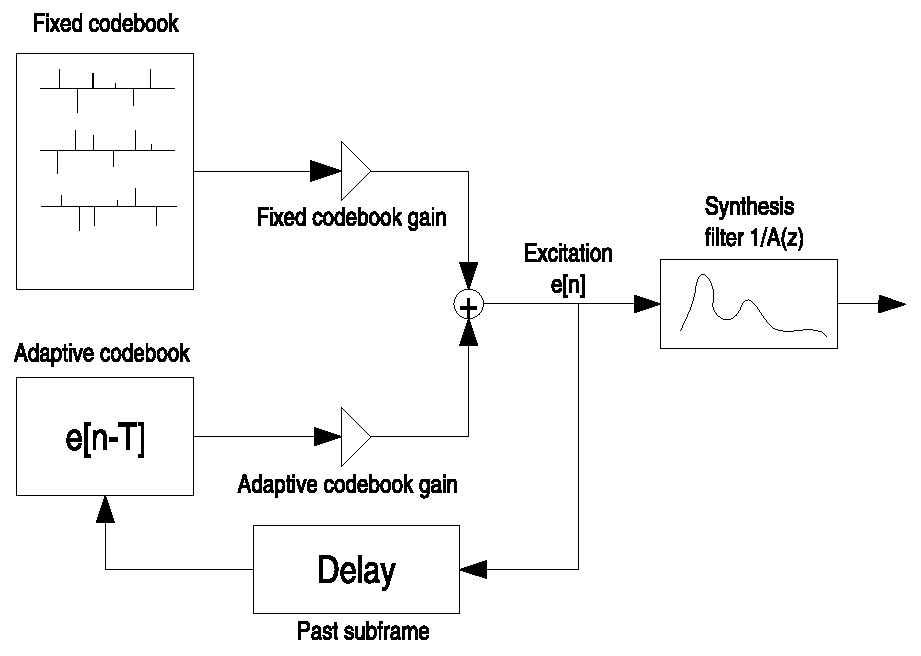
\includegraphics[width=0.45\paperwidth,keepaspectratio]{celp_decoder}\end{center}

\caption{Модель синтеза речи CELP (декодер)\label{fig:The-CELP-model} }
\end{figure}


\section{Коэффициенты линейного предсказания (LPC)\index{linear prediction}}

Линейное предсказание лежит в основе множества техник кодирования
речи, включая CELP. Идея заключается в том, что сигнал $x[n]$ предсказывается
с использованием линейной комбинации его выборок: 

\[
y[n]=\sum_{i=1}^{N}a_{i}x[n-i]
\]
 где $y[n]$ линейное предсказание$x[n]$. Таким образом, ошибка предсказания
представлена как:
\[
e[n]=x[n]-y[n]=x[n]-\sum_{i=1}^{N}a_{i}x[n-i]
\]
Цель линейного предсказания в том, чтобы найти наилучшие коэффициенты
предсказания $a_{i}$, при которых значение функции среднеквадратичной
ошибки является наименьшей:
\[
E=\sum_{n=0}^{L-1}\left[e[n]\right]^{2}=\sum_{n=0}^{L-1}\left[x[n]-\sum_{i=1}^{N}a_{i}x[n-i]\right]^{2}
\]
Это может быть осуществлено путем зануления производных $\frac{\partial E}{\partial a_{i}}$
:
\[
\frac{\partial E}{\partial a_{i}}=\frac{\partial}{\partial a_{i}}\sum_{n=0}^{L-1}\left[x[n]-\sum_{i=1}^{N}a_{i}x[n-i]\right]^{2}=0
\]

Для фильтра порядка $N$ коэффициенты $a_{i}$ могут быть найдены
с помощью решения системы линейных уравнений $\mathbf{Ra}=\mathbf{r}$
размерностью $N\times N$ , где
\[
\mathbf{R}=\left[\begin{array}{cccc}
R(0) & R(1) & \cdots & R(N-1)\\
R(1) & R(0) & \cdots & R(N-2)\\
\vdots & \vdots & \ddots & \vdots\\
R(N-1) & R(N-2) & \cdots & R(0)
\end{array}\right]
\]
\[
\mathbf{r}=\left[\begin{array}{c}
R(1)\\
R(2)\\
\vdots\\
R(N)
\end{array}\right]
\]
с $R(m)$, автокорреляцией\index{auto-correlation} сигнала $x[n]$,
вычисляемой по следующей формуле:

\[
R(m)=\sum_{i=0}^{N-1}x[i]x[i-m]
\]

Так как $\mathbf{R}$ самосопряженная матрица Тёплица, для решения
данной системы уравнений может быть использован алгоритм Левинсона-Дарбина
\index{Levinson-Durbin}, решающий эту задачу за $\mathcal{O}\left(N^{2}\right)$
итераций вместо $\mathcal{O}\left(N^{3}\right)$. Также может быть
доказано что все корни $A(z)$ находятся в пределах единичного круга,
это означает, что $1/A(z)$ всегда стабилен. Но это в теории, на практике
это не всегда является справедливым по причине конечной точности,
существуют две часто используемых техники, подтверждающие стабильность
фильтра. Во первых, можно умножить $R(0)$ на число немного большее
единицы (такое как 1.0001), что, в свою очередь, эквивалентно добавлению
шума к сигналу. Также мы можем применить оконную фильтрацию к автокорреляции,
что эквивалентно фильтрации в частотной области, уменьшающей острые
резонансы.

\section{Предсказание тембра\index{pitch}}

В течении звонких сегментов голосовой сигнал периодический, таким
образом, можно использовать это свойство путем аппроксимации сигнала
возбуждения $e[n]$, представляя его как усиленный в $\beta$ раз
предыдущий сигнал:

\[
e[n]\simeq p[n]=\beta e[n-T]\ ,
\]
где $T$ период основного тона, $\beta$ усиление основного тона.
Мы называем это долгосрочным предсказанием если источник предсказывается
как $e[n-T]$ с $T\gg N$.

\section{Инновационная кодовая таблица}

Последний сигнал возбуждения $e[n]$ будет являться суммой предсказанного
тона и инновационного сигнала $c[n]$, взятого из фиксированной кодовой
таблицы, отсюда и название линейное предсказание с \textit{мультикодовым}
управлением. Последнее выражение имеет вид:

\[
e[n]=p[n]+c[n]=\beta e[n-T]+c[n]\ .
\]
Квантование $c[n]$, где расположено большинство бит в CELP. Представляет
информацию, которая не может быть получена ни через линейное предсказание
ни через предсказание тона. В Z плоскости мы можем представить итоговый
сигнал $X(z)$ как 
\[
X(z)=\frac{C(z)}{A(z)\left(1-\beta z^{-T}\right)}
\]


\section{Взвешивание шума\index{error weighting}\index{analysis-by-synthesis}}

Большинство современных звуковых кодеков пытается сформировать шум
так, чтобы он отображался, в основном, в тех частотных областях, в
которых его не сможет распознать человеческое ухо. Для того, чтобы
максимизировать качество речи, CELP кодеки минимизируют среднеквадратичную
ошибку в перцепционно взвешенном домене. Это означает, что перцепционно
взвешенный шумовой фильтр $W(z)$ применяется к сигналу ошибки в кодировщике.
В большинстве CELP кодеков $W(z)$ это взвешивающий фильтр, полученный
из коэффициентов линейного предсказания, как правило с помощью расширения
полосы частот. Предположим, что огибающая спектра представлена синтезирующим
фильтром $1/A(z)$, тогда в CELP кодеках полученный взвешивающий фильтр
шумов обычно представлен как: 
\begin{equation}
W(z)=\frac{A(z/\gamma_{1})}{A(z/\gamma_{2})}\ ,\label{eq:gamma-weighting}
\end{equation}
где $\gamma_{1}=0.9$ и $\gamma_{2}=0.6$ в базовой реализации Speex.
Если фильтр $A(z)$ имеет комплексные полюса $p_{i}$ на $z$-плоскости,
фильтр $A(z/\gamma)$ будет иметь полюса $p'_{i}=\gamma p_{i}$, таким
образом добиваясь более плоского варианта $A(z)$.

Взвешивающий фильтр применяется к сигналу ошибок для оптимизации поиска
по кодовой таблице при анализе через синтез (Analysis-by-Synthesis
или AbS). Это приводит к определенному результату в спектре шума,
который стремится к $1/W(z)$. Пока простота модели является важной
причиной успеха CELP, остается, что $W(z)$ это очень грубая аппроксимация
для функции перцепционно оптимального взвешивания шума. Рисунок \ref{cap:Standard-noise-shaping}
показывает сглаживание шума, полученное с помощью выражения \ref{eq:gamma-weighting}.
Во всем данном руководстве под $W(z)$ мы подразумеваем взвешивающий
фильтр шума и под $1/W(z)$ мы подразумеваем формирующий шумовой фильтр
(или кривая).

\begin{figure}
\begin{center}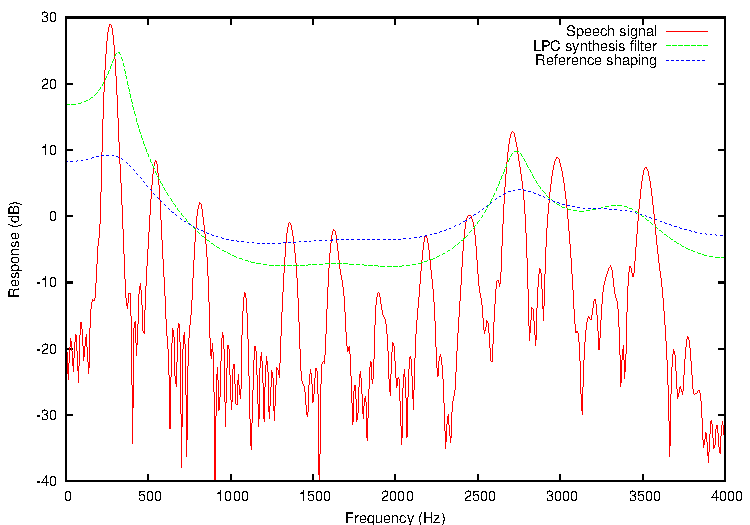
\includegraphics[width=0.45\paperwidth,keepaspectratio]{ref_shaping}\end{center}

\caption{Стандартное подавление шума в CELP. Произвольное смещение оси y.\label{cap:Standard-noise-shaping}}
\end{figure}


\section{Анализ через синтез}

Один из основных принципов CELP назван анализом через синтез (AbS),
это означает, что кодирование (анализ) осуществляется с помощью перцепционной
оптимизации декодированного (синтез) сигнала в замкнутом цикле. В
теории лучший CELP поток должен быть произведен путем проверки всех
возможных комбинаций битов и выбора одной, которая воспроизведет декодированный
сигнал, звучащий наилучшим образом. Очевидно, что это не реализуемо
на практике по двум причинам: требуемая сложность намного выше возможностей
доступного на данный момент аппаратного обеспечения и критерий выбора
наилучшего звучания определяется слушателем. 

С целью достижения кодирования в реальном времени с использованием
ограниченных вычислительных ресурсов, оптимизация разбивается на меньшие,
более управляемые, последовательные поиски с использованием взвешивающей
функции, описанной ранее.

\newpage{}

\chapter{Узкополосный режим Speex\label{sec:Speex-narrowband-mode}\index{narrowband}}

Данный раздел рассматривает то, как работает Speex в узкополосном
(частота дискретизации $8\:\mathrm{\text{кГц}}$) режиме. Размер
кадра для данного режима равен $20\:\mathrm{\text{мс}}$, что соответствует
160 выборкам. Каждый кадр разделяется на 4 подкадра по 40 выборок
каждый.

Также большинство решений проектирования было основано на первоначальных
целях и предположениях:
\begin{itemize}
\item Минимизация количества информации, извлекаемой из предыдущих кадров
(для стойкости к потере пакетов)
\item Динамически выбираемые кодовые таблицы (LSP, шаговые и инновационные)
\item Кодовые таблицы с фиксированным субвектором (инновационные)
\end{itemize}

\section{Анализ кадра целиком\index{linear prediction}}

В узкополосном режиме, кадры Speex длиной в 20 мс (160 выборок) и
разделены на 4 субкадра по 5 мс каждый (40 выборок). Для большинства
узкополосных битрейтов (8 кбит/с и выше) параметры, кодируемые только
на уровне кадра, это линейные спектральные пары (LSP) и глобальное
усиление сигнала возбуждения $g_{frame}$, как показано на рисунке
\ref{cap:Frame-open-loop-analysis}. Все остальные параметры кодируются
на уровне субкадров.

Анализ линейного предсказания осуществляется один раз за кадр с использованием
асимметричного окна Хемминга, центрированного по четверти субкадра.
Потому что коэффициенты линейного предсказания (LPC) квантуются не
сразу, сначала они конвертируются в линейные спектральные пары (LSP)\index{line spectral pair}.
Считается что коэффициенты LSP связаны с четвертью субкадров, и коэффициенты,
связанные с первыми тремя субкадрами, линейно интерполируются с использованием
текущего и предыдущего коэффициента LSP. Полученные коэффициенты конвертируются
обратно в коэффициенты LPC фильтра $\hat{A}(z)$. Не квантованный
интерполированный фильтр представлен как $A(z)$ и может быть использован
для взвешивающего фильтра $W(z)$, потому как нет необходимости в
доступности данного фильтра для декодировщика.

Для того, чтобы сделать Speex более стойким к потере пакетов, к коэффициентам
LSP не применяется предсказание до квантования. Коэффициенты LSP кодируются
с помощью векторного квантования (VQ) с 30 битами для более высокого
качества и 18 битами для более низкого качества.

\begin{figure}
\begin{center}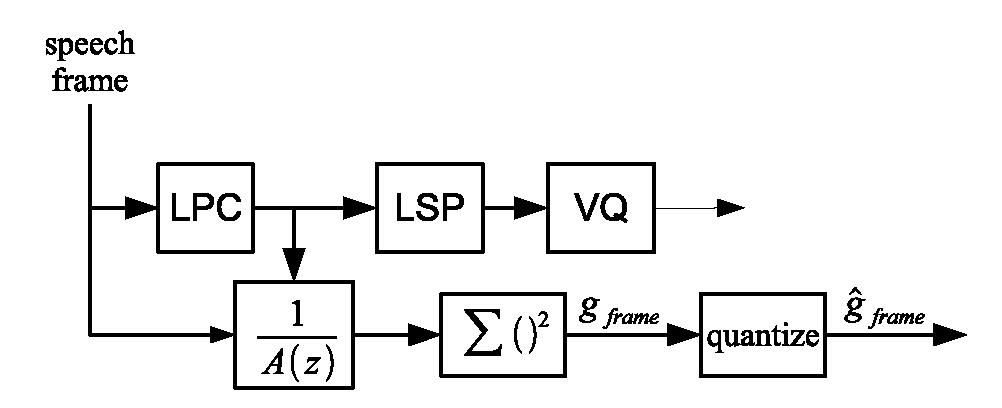
\includegraphics[width=0.35\paperwidth]{speex_analysis}\end{center}

\caption{Анализ кадра в разомкнутом контуре\label{cap:Frame-open-loop-analysis}}
\end{figure}


\section{Анализ через синтез субкадров}

\begin{figure}
\begin{center}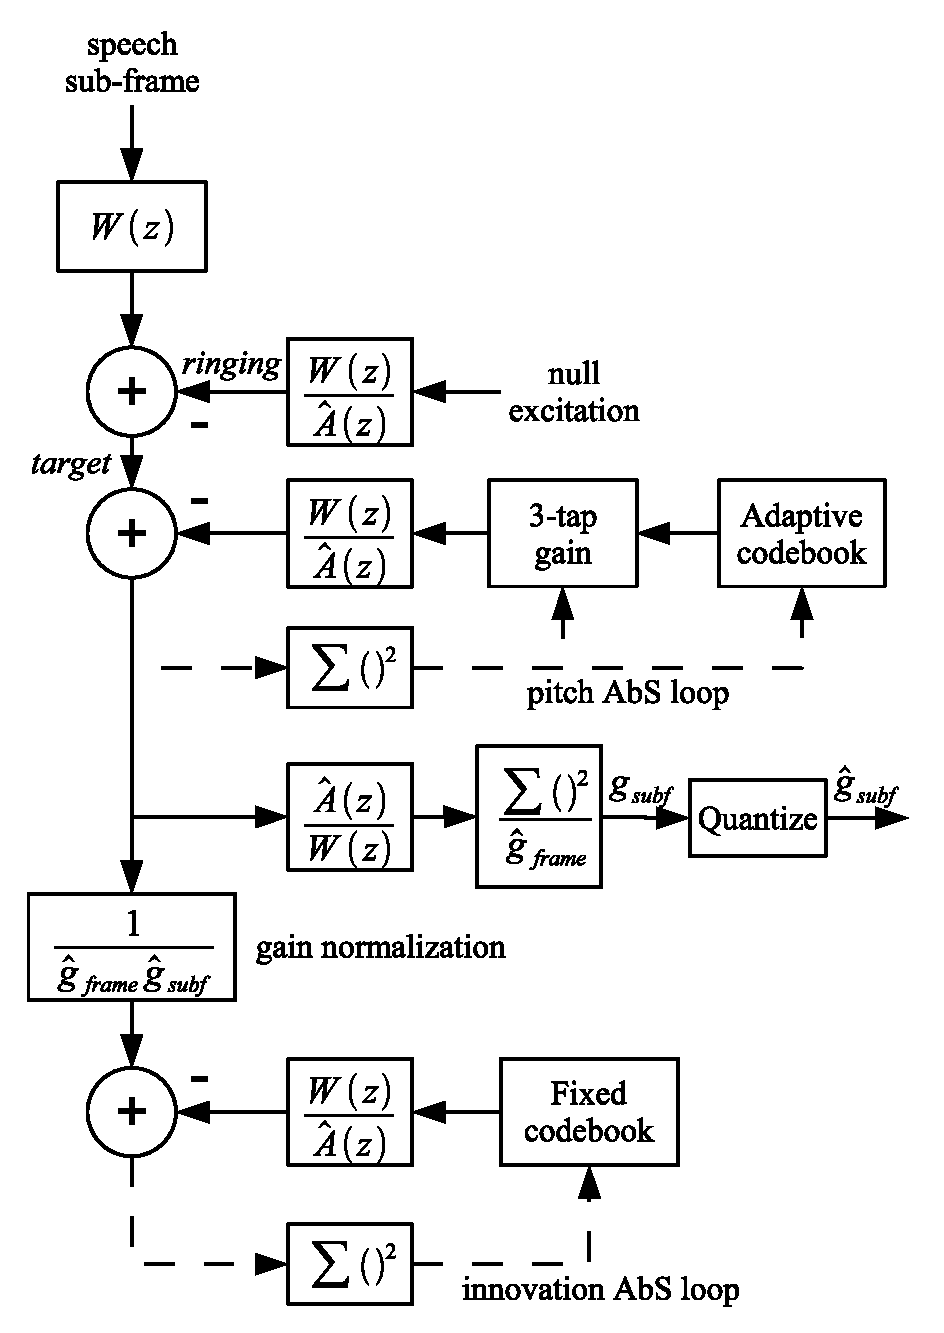
\includegraphics[width=0.4\paperwidth]{speex_abs}\end{center}

\caption{Оптимизация субкадра анализом через синтез в замкнутом цикле.\label{cap:Sub-frame-AbS}}
\end{figure}

Цикл кодировщика анализа через синтез показан на рисунке \ref{cap:Sub-frame-AbS}.
Существуют три основных аспекта по которым Speex значительно отличается
большинства остальных CELP кодировщиков. Во-первых, пока большинство
новых CELP кодировщиков используют дробную оценку тембра с одним коэффициентом
усиления , Speex использует целое число для кодирования периода тембра,
но использует предсказание с тремя коэффициентами усиления. Роль адаптивной
кодовой таблицы $e_{a}[n]$ может быть представлено как:
\begin{equation}
e_{a}[n]=g_{0}e[n-T-1]+g_{1}e[n-T]+g_{2}e[n-T+1]\label{eq:adaptive-3tap}
\end{equation}
где $g_{0}$, $g_{1}$ и $g_{2}$ это совместно квантованные коэффициенты
усиления тембра и $e[n]$ это сигнал возбуждения в памяти кодека.
Стоит заметить, что когда длина участка с одинаковым тембром меньше
длины субкадра, мы повторяем сигнал возбуждения на период $T$. Например,
когда $n-T+1\geq0$, мы используем $n-2T+1$ вместо этого. В большинстве
режимов период тембра кодируется семью битами в диапазоне $\left[17,144\right]$
и коэффициенты $\beta_{i}$ квантованы векторно с 7 битами на более
высоких битрейтах (15 кбит/с в узкополосном режиме и более) и пятью
на более низких (11 кбит/с в узкополосном режиме и менее).

Большинство существующих на данный момент CELP кодеков используют
предсказание со скользящим средним (MA) для кодирования коэффициента
усиления из фиксированной кодовой таблицы. Это предоставляет немного
лучшее кодирование ценой введения зависимости от ранее закодированных
кадров. Второе отличие состоит в том, что Speex кодирует коэффициент
усиления как продукт глобального усиления сигнала возбуждения $g_{frame}$
с поправками усиления субкадра $g_{subf}$. Это увеличивает стойкость
к потере пакетов путем уничтожения межкадровой зависимости. Коэффициент
усиления субкадра кодируется до поиска в фиксированной таблице (оптимизация
без обратной связи) и использует между 0 и 3 битами на субкадр, в
зависимости от битрейта.

Третье различие состоит в том, что Speex использует субвекторное квантование
для инновационного (с фиксированной таблицей) сигнала вместо алгебраической
кодовой таблицы. Каждый субкадр разделен на субвекторы длины, варьирующейся
между 5 и 20 выборками. Каждый субвектор выбирается из кодовой таблицы,
зависимой от битрейта, и все субвекторы склеиваются для того, чтобы
сформировать субкадр. В качестве примера, режим с 3.95 кбит/с использует
размер субвектора в 20 выборок с 32 записями в кодовой таблице (5
бит). Это означает, что инновационный сигнал кодируется с 10 битами
на субкадр, или 2000 бит/с. С другой стороны, в режиме 18.2 кбит/с
используется размер субвектора из 5 выборок с 256 записями в кодовой
таблице (8 bits), то есть инновационный сигнал использует 64 бита
на субкадр, или 12800 бит/с. 

\section{Битрейты}

До сих пор нет MOS (абсолютно субъективного понятия\index{mean opinion score}),
но субъективная оценка была проведена для Speex. Для того, чтобы дать
общее представление о качестве, достижимом с помощью данного кодека,
таблица \ref{cap:quality_vs_bps} представляет мое субъективное мнение
об этом. Следует заметить, что разные люди воспринимают качество по
разному и человек, создавший этот кодек, имел некоторую предвзятость
при субъективной оценке. Последнее, что следует упомянуть, это то,
что качество большинства кодеков (включая Speex) варьируется в зависимости
от входного сигнала. Обратите внимание, что сложность только приблизительная
(с 0.5 мфлопс и использованием наименьшей установки сложности). Для
декодирования требуется приблизительно 0.5 мфлопс \index{complexity}
в большинстве режимов (1 мфлопс с перцепционным усилением).

\begin{table*}[h]
\begin{center}%
\begin{tabular}{|c|c|c|c|c|}
\hline 
Режим & Качество & Битрейт\index{bit-rate} (бит/с) & мфлоп\index{complexity} & Качество/описание\tabularnewline
\hline 
\hline 
0 & - & 250 & 0 & Нет передачи (DTX)\tabularnewline
\hline 
1 & 0 & 2,150 & 6 & Вокодер (в основном для комфортного шума)\tabularnewline
\hline 
2 & 2 & 5,950 & 9 & Очень заметные артефакты/шум, хорошая разборчивость\tabularnewline
\hline 
3 & 3-4 & 8,000 & 10 & Артефакты/шум иногда заметны\tabularnewline
\hline 
4 & 5-6 & 11,000 & 14 & Артефакты иногда заметны только в наушниках\tabularnewline
\hline 
5 & 7-8 & 15,000 & 11 & Нужны хорошие наушники для того, чтобы заметить разницу\tabularnewline
\hline 
6 & 9 & 18,200 & 17.5 & Трудно заметить разницу даже в хороших наушниках\tabularnewline
\hline 
7 & 10 & 24,600 & 14.5 & Полностью прозрачен для голоса, хорошее качество музыки\tabularnewline
\hline 
8 & 1 & 3,950 & 10.5 & Очень заметные артефакты/шум, хорошая разборчивость\tabularnewline
\hline 
9 & - & - & - & зарезервировано\tabularnewline
\hline 
10 & - & - & - & зарезервировано\tabularnewline
\hline 
11 & - & - & - & зарезервировано\tabularnewline
\hline 
12 & - & - & - & зарезервировано\tabularnewline
\hline 
13 & - & - & - & Определяется реализацией, интерпретируется вызовом функции или пропускается\tabularnewline
\hline 
14 & - & - & - & Внутриполосная связь Speex\tabularnewline
\hline 
15 & - & - & - & Код разделителя\tabularnewline
\hline 
\end{tabular}\end{center}

\caption{Качество в сравнении с битрейтом\label{cap:quality_vs_bps}}
\end{table*}


\section{Перцепционное усиление\index{perceptual enhancement}}

\textbf{Данный раздел действителен только для версии 1.1.12 и более
ранних. Он не применим к версии 1.2-beta1 (и поздних), для которых
новое перцепционное усиление до сих пор не задокументировано.}

Данная часть кодека применяется только к декодировщику и даже может
быть изменена без нарушения функциональной совместимости. По этой
причине, реализация предоставленная и описанная здесь должна рассматриваться
только как пример реализации. Усиление разделено на две части. Первая,
это синтезирующий фильтр$S(z)=1/A(z)$ заменен улучшенным фильтром:
\[
S'(z)=\frac{A\left(z/a_{2}\right)A\left(z/a_{3}\right)}{A\left(z\right)A\left(z/a_{1}\right)}
\]
где $a_{1}$ и $a_{2}$ зависят от используемого режима и $a_{3}=\frac{1}{r}\left(1-\frac{1-ra_{1}}{1-ra_{2}}\right)$
с $r=.9$. Вторая часть усиления состоит из использования гребенчатого
фильтра для того, чтобы улучшить шаг в области сигнала возбуждения. 

\newpage{}

\chapter{Широкополосный режим Speex (поддиапазон CELP)\index{wideband}\label{sec:Speex-wideband-mode}}

Для широкополосного режима, Speex использует квадратурный зеркальный
фильтр\index{quadrature mirror filter} (QMF) для того чтобы расколоть
диапазон на два. Таким образом сигнал частотой 16 кГц разделяется
на два сигнала частотой 8 кГц, один представляет нижний диапазон (0-4
кГц), другой верхний диапазон (4-8 кГц). Нижний диапазон кодируется
в узкополосном режиме, описанном в разделе \ref{sec:Speex-narrowband-mode},
таким образом, полученный ``встроенный узкополосный поток'' также
может быть декодирован узкополосным декодировщиком. Т. к. кодирование
нижнего диапазона уже описано, в данном разделе будет рассматриваться
только кодирование верхнего диапазона.

\section{Линейное предсказание}

Линейное предсказание для верхнего диапазона очень похоже на то, что
использовалось для узкополосного режима. Единственная разница в, том
что мы используем только 12 бит для кодирования LPS верхнего поддиапазона,
используя многоступенчатый векторный квантователь (MSVQ). Первый уровень
квантуется 10 коэффициентами с 6 битами и ошибкой, которая после квантуется
с использованием так же 6 бит.

\section{Предсказание тембра}

Эта часть описания простая: нет никакого предсказания тембра для верхнего
поддиапазона. На то существуют две причины. Во-первых, гармоническая
структура обычно слабо выражена в этом диапазоне (выше 4 кГц). Во-вторых,
это было бы очень трудно реализовать так как QMF загибает диапазон
4-8 кГц в 4-0 кГц (переворачивая частотную ось), это означает, что
гармоники больше не расположены на частотах кратных фундаментальным
(тембру). 

\section{Квантование сигнала возбуждения}

Сигнал возбуждения верхнего диапазона кодируется так же, как и сигнал
в узкополосном режиме. 

\section{Расположение битов}

Для широкополосного режима внутренний узкополосный кадр пакуется до
того, как кодируется верхний поддиапазон. Верхний поддиапазон расположен,
как показано в таблице \ref{cap:bits-wideband}. Для широкополосного
режима, ID режима такой же как и установка качества Speex, определенная
в таблице \ref{tab:wideband-quality}. Это также означает, что широкополосный
кадр может быть декодирован узкополосным декодировщиком только с одним
предостережением, состоящем в том, что в одном пакете может быть более
одного кадра, декодировщику будет необходимо пропускать широкополосные
части для синхронизации битового потока.

\begin{table*}[h]
\begin{center}%
\begin{tabular}{|c|c|c|c|c|c|c|}
\hline 
Параметр & Частота обновления & 0 & 1 & 2 & 3 & 4\tabularnewline
\hline 
\hline 
Широкополосный бит & кадр & 1 & 1 & 1 & 1 & 1\tabularnewline
\hline 
ID режима & кадр & 3 & 3 & 3 & 3 & 3\tabularnewline
\hline 
LSP & кадр & 0 & 12 & 12 & 12 & 12\tabularnewline
\hline 
Усиление сигнала возбуждения & субкадр & 0 & 5 & 4 & 4 & 4\tabularnewline
\hline 
Excitation VQ & субкадр & 0 & 0 & 20 & 40 & 80\tabularnewline
\hline 
\hline 
Итог & кадр & 4 & 36 & 112 & 192 & 352\tabularnewline
\hline 
\end{tabular}\end{center}

\caption{Расположение бит для верхнего диапазона в широкополосном режиме\label{cap:bits-wideband}}
\end{table*}

\begin{table*}[h]
\begin{center}%
\begin{tabular}{|c|c|c|}
\hline 
Режим/качество & Битрейт\index{bit-rate} (кбит/с) & Качество/описание\tabularnewline
\hline 
\hline 
0 & 3,950 & Едва понятный (главным образом для комфортного шума)\tabularnewline
\hline 
1 & 5,750 & Очень заметные артефакты/шум, плохая различимость\tabularnewline
\hline 
2 & 7,750 & Очень заметные артефакты/шум, хорошая различимость\tabularnewline
\hline 
3 & 9,800 & Артефакты/шум иногда надоедливы\tabularnewline
\hline 
4 & 12,800 & Артефакты/шум обычно заметны\tabularnewline
\hline 
5 & 16,800 & Артефакты/шум иногда заметны\tabularnewline
\hline 
6 & 20,600 & Нужны хорошие наушники для того, чтобы заметить разницу\tabularnewline
\hline 
7 & 23,800 & Нужны хорошие наушники для того, чтобы заметить разницу\tabularnewline
\hline 
8 & 27,800 & Трудно заметить разницу даже в хороших наушниках\tabularnewline
\hline 
9 & 34,200 & Трудно заметить разницу даже в хороших наушниках\tabularnewline
\hline 
10 & 42,200 & Полностью прозрачен для голоса, хорошее качество музыки\tabularnewline
\hline 
\end{tabular}\end{center}

\caption{Соотношение качества и битрейта для широкополосного кодировщика\label{tab:wideband-quality}}
\end{table*}

\clearpage

\clearpage

\appendix

\chapter{Примеры кода\label{sec:Sample-code}}

Данный раздел показывает пример кода для кодирования и декодирования
речи с использованием Speex API. Команды, используемые для кодирование
и декодирования файла могут быть следующими:\texttt{}~\\
\texttt{\% sampleenc in\_file.sw \textbar{} sampledec out\_file.sw}\\
где оба файла сырые (без заголовка) закодированные при 16 битах на
выборку (с естественным машинным порядком байт).

\section{sampleenc.c}

sampleenc принимает сырой файл с 16 битами на выборку, кодирует его
и выдает поток Speex в stdout. Заметьте что используемый здесь формат
файла несовместим с speexenc/speexdec.

\lstinputlisting[numbers=left,numberstyle={\footnotesize},caption={Source code for sampleenc},label={sampleenc-source-code}]{sampleenc.c}

\section{sampledec.c}

sampledec считывает Speex поток из stdin, декодирует его, и выдает
в файл с 16 битами на семпл. Заметьте что используемый здесь формат
файла несовместим с speexenc/speexdec.

\lstinputlisting[numbers=left,numberstyle={\footnotesize},caption={Source code for sampledec},label={sampledec-source-code}]{sampledec.c}

\newpage{}

\chapter{IETF RTP профиль\label{sec:IETF-draft}}

\verbatiminput{draft-ietf-avt-rtp-speex-05-tmp.txt}

\newpage{}

\chapter{Лицензия Speex\label{sec:Speex-License}}

\verbatiminput{../COPYING}

\newpage{}

\chapter{GNU Free Documentation License}

Version 1.1, March 2000

Copyright (C) 2000 Free Software Foundation, Inc. 59 Temple Place,
Suite 330, Boston, MA 02111-1307 USA Everyone is permitted to copy
and distribute verbatim copies of this license document, but changing
it is not allowed. 

\section*{0. PREAMBLE}

The purpose of this License is to make a manual, textbook, or other
written document \textquotedbl free\textquotedbl{} in the sense of
freedom: to assure everyone the effective freedom to copy and redistribute
it, with or without modifying it, either commercially or noncommercially.
Secondarily, this License preserves for the author and publisher a
way to get credit for their work, while not being considered responsible
for modifications made by others.

This License is a kind of \textquotedbl copyleft\textquotedbl ,
which means that derivative works of the document must themselves
be free in the same sense. It complements the GNU General Public License,
which is a copyleft license designed for free software.

We have designed this License in order to use it for manuals for free
software, because free software needs free documentation: a free program
should come with manuals providing the same freedoms that the software
does. But this License is not limited to software manuals; it can
be used for any textual work, regardless of subject matter or whether
it is published as a printed book. We recommend this License principally
for works whose purpose is instruction or reference. 

\section*{1. APPLICABILITY AND DEFINITIONS}

This License applies to any manual or other work that contains a notice
placed by the copyright holder saying it can be distributed under
the terms of this License. The \textquotedbl Document\textquotedbl ,
below, refers to any such manual or work. Any member of the public
is a licensee, and is addressed as \textquotedbl you\textquotedbl .

A \textquotedbl Modified Version\textquotedbl{} of the Document means
any work containing the Document or a portion of it, either copied
verbatim, or with modifications and/or translated into another language.

A \textquotedbl Secondary Section\textquotedbl{} is a named appendix
or a front-matter section of the Document that deals exclusively with
the relationship of the publishers or authors of the Document to the
Document's overall subject (or to related matters) and contains nothing
that could fall directly within that overall subject. (For example,
if the Document is in part a textbook of mathematics, a Secondary
Section may not explain any mathematics.) The relationship could be
a matter of historical connection with the subject or with related
matters, or of legal, commercial, philosophical, ethical or political
position regarding them.

The \textquotedbl Invariant Sections\textquotedbl{} are certain Secondary
Sections whose titles are designated, as being those of Invariant
Sections, in the notice that says that the Document is released under
this License.

The \textquotedbl Cover Texts\textquotedbl{} are certain short passages
of text that are listed, as Front-Cover Texts or Back-Cover Texts,
in the notice that says that the Document is released under this License.

A \textquotedbl Transparent\textquotedbl{} copy of the Document means
a machine-readable copy, represented in a format whose specification
is available to the general public, whose contents can be viewed and
edited directly and straightforwardly with generic text editors or
(for images composed of pixels) generic paint programs or (for drawings)
some widely available drawing editor, and that is suitable for input
to text formatters or for automatic translation to a variety of formats
suitable for input to text formatters. A copy made in an otherwise
Transparent file format whose markup has been designed to thwart or
discourage subsequent modification by readers is not Transparent.
A copy that is not \textquotedbl Transparent\textquotedbl{} is called
\textquotedbl Opaque\textquotedbl .

Examples of suitable formats for Transparent copies include plain
ASCII without markup, Texinfo input format, \LaTeX{} input format,
SGML or XML using a publicly available DTD, and standard-conforming
simple HTML designed for human modification. Opaque formats include
PostScript, PDF, proprietary formats that can be read and edited only
by proprietary word processors, SGML or XML for which the DTD and/or
processing tools are not generally available, and the machine-generated
HTML produced by some word processors for output purposes only.

The \textquotedbl Title Page\textquotedbl{} means, for a printed
book, the title page itself, plus such following pages as are needed
to hold, legibly, the material this License requires to appear in
the title page. For works in formats which do not have any title page
as such, \textquotedbl Title Page\textquotedbl{} means the text near
the most prominent appearance of the work's title, preceding the beginning
of the body of the text.

\section*{2. VERBATIM COPYING}

You may copy and distribute the Document in any medium, either commercially
or noncommercially, provided that this License, the copyright notices,
and the license notice saying this License applies to the Document
are reproduced in all copies, and that you add no other conditions
whatsoever to those of this License. You may not use technical measures
to obstruct or control the reading or further copying of the copies
you make or distribute. However, you may accept compensation in exchange
for copies. If you distribute a large enough number of copies you
must also follow the conditions in section 3.

You may also lend copies, under the same conditions stated above,
and you may publicly display copies.

\section*{3. COPYING IN QUANTITY}

If you publish printed copies of the Document numbering more than
100, and the Document's license notice requires Cover Texts, you must
enclose the copies in covers that carry, clearly and legibly, all
these Cover Texts: Front-Cover Texts on the front cover, and Back-Cover
Texts on the back cover. Both covers must also clearly and legibly
identify you as the publisher of these copies. The front cover must
present the full title with all words of the title equally prominent
and visible. You may add other material on the covers in addition.
Copying with changes limited to the covers, as long as they preserve
the title of the Document and satisfy these conditions, can be treated
as verbatim copying in other respects.

If the required texts for either cover are too voluminous to fit legibly,
you should put the first ones listed (as many as fit reasonably) on
the actual cover, and continue the rest onto adjacent pages.

If you publish or distribute Opaque copies of the Document numbering
more than 100, you must either include a machine-readable Transparent
copy along with each Opaque copy, or state in or with each Opaque
copy a publicly-accessible computer-network location containing a
complete Transparent copy of the Document, free of added material,
which the general network-using public has access to download anonymously
at no charge using public-standard network protocols. If you use the
latter option, you must take reasonably prudent steps, when you begin
distribution of Opaque copies in quantity, to ensure that this Transparent
copy will remain thus accessible at the stated location until at least
one year after the last time you distribute an Opaque copy (directly
or through your agents or retailers) of that edition to the public.

It is requested, but not required, that you contact the authors of
the Document well before redistributing any large number of copies,
to give them a chance to provide you with an updated version of the
Document. 

\section*{4. MODIFICATIONS}

You may copy and distribute a Modified Version of the Document under
the conditions of sections 2 and 3 above, provided that you release
the Modified Version under precisely this License, with the Modified
Version filling the role of the Document, thus licensing distribution
and modification of the Modified Version to whoever possesses a copy
of it. In addition, you must do these things in the Modified Version: 
\begin{itemize}
\item A. Use in the Title Page (and on the covers, if any) a title distinct
from that of the Document, and from those of previous versions (which
should, if there were any, be listed in the History section of the
Document). You may use the same title as a previous version if the
original publisher of that version gives permission.
\item B. List on the Title Page, as authors, one or more persons or entities
responsible for authorship of the modifications in the Modified Version,
together with at least five of the principal authors of the Document
(all of its principal authors, if it has less than five).
\item C. State on the Title page the name of the publisher of the Modified
Version, as the publisher.
\item D. Preserve all the copyright notices of the Document.
\item E. Add an appropriate copyright notice for your modifications adjacent
to the other copyright notices.
\item F. Include, immediately after the copyright notices, a license notice
giving the public permission to use the Modified Version under the
terms of this License, in the form shown in the Addendum below.
\item G. Preserve in that license notice the full lists of Invariant Sections
and required Cover Texts given in the Document's license notice.
\item H. Include an unaltered copy of this License.
\item I. Preserve the section entitled \textquotedbl History\textquotedbl ,
and its title, and add to it an item stating at least the title, year,
new authors, and publisher of the Modified Version as given on the
Title Page. If there is no section entitled \textquotedbl History\textquotedbl{}
in the Document, create one stating the title, year, authors, and
publisher of the Document as given on its Title Page, then add an
item describing the Modified Version as stated in the previous sentence.
\item J. Preserve the network location, if any, given in the Document for
public access to a Transparent copy of the Document, and likewise
the network locations given in the Document for previous versions
it was based on. These may be placed in the \textquotedbl History\textquotedbl{}
section. You may omit a network location for a work that was published
at least four years before the Document itself, or if the original
publisher of the version it refers to gives permission.
\item K. In any section entitled \textquotedbl Acknowledgements\textquotedbl{}
or \textquotedbl Dedications\textquotedbl , preserve the section's
title, and preserve in the section all the substance and tone of each
of the contributor acknowledgements and/or dedications given therein.
\item L. Preserve all the Invariant Sections of the Document, unaltered
in their text and in their titles. Section numbers or the equivalent
are not considered part of the section titles.
\item M. Delete any section entitled \textquotedbl Endorsements\textquotedbl .
Such a section may not be included in the Modified Version.
\item N. Do not retitle any existing section as \textquotedbl Endorsements\textquotedbl{}
or to conflict in title with any Invariant Section. 
\end{itemize}
If the Modified Version includes new front-matter sections or appendices
that qualify as Secondary Sections and contain no material copied
from the Document, you may at your option designate some or all of
these sections as invariant. To do this, add their titles to the list
of Invariant Sections in the Modified Version's license notice. These
titles must be distinct from any other section titles.

You may add a section entitled \textquotedbl Endorsements\textquotedbl ,
provided it contains nothing but endorsements of your Modified Version
by various parties--for example, statements of peer review or that
the text has been approved by an organization as the authoritative
definition of a standard.

You may add a passage of up to five words as a Front-Cover Text, and
a passage of up to 25 words as a Back-Cover Text, to the end of the
list of Cover Texts in the Modified Version. Only one passage of Front-Cover
Text and one of Back-Cover Text may be added by (or through arrangements
made by) any one entity. If the Document already includes a cover
text for the same cover, previously added by you or by arrangement
made by the same entity you are acting on behalf of, you may not add
another; but you may replace the old one, on explicit permission from
the previous publisher that added the old one.

The author(s) and publisher(s) of the Document do not by this License
give permission to use their names for publicity for or to assert
or imply endorsement of any Modified Version. 

\section*{5. COMBINING DOCUMENTS}

You may combine the Document with other documents released under this
License, under the terms defined in section 4 above for modified versions,
provided that you include in the combination all of the Invariant
Sections of all of the original documents, unmodified, and list them
all as Invariant Sections of your combined work in its license notice.

The combined work need only contain one copy of this License, and
multiple identical Invariant Sections may be replaced with a single
copy. If there are multiple Invariant Sections with the same name
but different contents, make the title of each such section unique
by adding at the end of it, in parentheses, the name of the original
author or publisher of that section if known, or else a unique number.
Make the same adjustment to the section titles in the list of Invariant
Sections in the license notice of the combined work.

In the combination, you must combine any sections entitled \textquotedbl History\textquotedbl{}
in the various original documents, forming one section entitled \textquotedbl History\textquotedbl ;
likewise combine any sections entitled \textquotedbl Acknowledgements\textquotedbl ,
and any sections entitled \textquotedbl Dedications\textquotedbl .
You must delete all sections entitled \textquotedbl Endorsements.\textquotedbl{}

\section*{6. COLLECTIONS OF DOCUMENTS}

You may make a collection consisting of the Document and other documents
released under this License, and replace the individual copies of
this License in the various documents with a single copy that is included
in the collection, provided that you follow the rules of this License
for verbatim copying of each of the documents in all other respects.

You may extract a single document from such a collection, and distribute
it individually under this License, provided you insert a copy of
this License into the extracted document, and follow this License
in all other respects regarding verbatim copying of that document. 

\section*{7. AGGREGATION WITH INDEPENDENT WORKS}

A compilation of the Document or its derivatives with other separate
and independent documents or works, in or on a volume of a storage
or distribution medium, does not as a whole count as a Modified Version
of the Document, provided no compilation copyright is claimed for
the compilation. Such a compilation is called an \textquotedbl aggregate\textquotedbl ,
and this License does not apply to the other self-contained works
thus compiled with the Document, on account of their being thus compiled,
if they are not themselves derivative works of the Document.

If the Cover Text requirement of section 3 is applicable to these
copies of the Document, then if the Document is less than one quarter
of the entire aggregate, the Document's Cover Texts may be placed
on covers that surround only the Document within the aggregate. Otherwise
they must appear on covers around the whole aggregate.

\section*{8. TRANSLATION}

Translation is considered a kind of modification, so you may distribute
translations of the Document under the terms of section 4. Replacing
Invariant Sections with translations requires special permission from
their copyright holders, but you may include translations of some
or all Invariant Sections in addition to the original versions of
these Invariant Sections. You may include a translation of this License
provided that you also include the original English version of this
License. In case of a disagreement between the translation and the
original English version of this License, the original English version
will prevail.

\section*{9. TERMINATION}

You may not copy, modify, sublicense, or distribute the Document except
as expressly provided for under this License. Any other attempt to
copy, modify, sublicense or distribute the Document is void, and will
automatically terminate your rights under this License. However, parties
who have received copies, or rights, from you under this License will
not have their licenses terminated so long as such parties remain
in full compliance. 

\section*{10. FUTURE REVISIONS OF THIS LICENSE}

The Free Software Foundation may publish new, revised versions of
the GNU Free Documentation License from time to time. Such new versions
will be similar in spirit to the present version, but may differ in
detail to address new problems or concerns. See http://www.gnu.org/copyleft/.

Each version of the License is given a distinguishing version number.
If the Document specifies that a particular numbered version of this
License \textquotedbl or any later version\textquotedbl{} applies
to it, you have the option of following the terms and conditions either
of that specified version or of any later version that has been published
(not as a draft) by the Free Software Foundation. If the Document
does not specify a version number of this License, you may choose
any version ever published (not as a draft) by the Free Software Foundation.

\printindex
\end{document}
